\documentclass[a4paper, 12pt]{report}

\title{Конспект лекций по математическому анализу 2023/2024}
\author{Корчагин Егор}
\date { \today }

\usepackage[english, russian]{babel}
\usepackage[T2A]{fontenc}
\usepackage[utf8]{inputenc}
\usepackage{indentfirst}

\usepackage{xr, amsmath, amsfonts, amssymb, amsthm, mathtools, mathtext}

\newtheorem{theorem}{Теорема}[chapter]
\newtheorem{lemma}[theorem]{Лемма}
\newtheorem{mention}[theorem]{Замечание}
\newtheorem{corollary}[theorem]{Следствие}
\newtheorem{definition}[theorem]{Определение}
\newtheorem{example}[theorem]{Пример}
\newtheorem{sentence}[theorem]{Предложение}
\newtheorem*{explanation}{Пояснение}

\usepackage{geometry}
\geometry{top=25mm}
\geometry{bottom=30mm}
\geometry{left=15mm}
\geometry{right=15mm}

\usepackage{titleps}
\newpagestyle{main}{
	\setheadrule{0.4pt}
	\sethead{НИУ ВШЭ}{}{Корчагин Егор}
	\setfootrule{0.4pt}
	\setfoot{Конспект лекций по математическому анализу 2023/2024}{}{\thepage}
}
\pagestyle{main}

\usepackage{soulutf8}

\newcommand{\deriv}[2]{\frac{\partial #1}{\partial #2}}
\newcommand{\R}{\mathbb R}
\newcommand{\Z}{\mathbb Z}
\newcommand{\N}{\mathbb N}
\newcommand{\Q}{\mathbb Q}
\newcommand{\I}{\mathbb I}

\renewcommand{\phi}{\varphi}
\renewcommand{\epsilon}{\varepsilon}
\renewcommand{\kappa}{\varkappa}

\DeclareMathOperator{\Kerr}{Ker}
\DeclareMathOperator{\Imm}{Im}

\DeclareMathOperator*{\argmax}{argmax}

\newcommand{\percent}{\mathbin{\%}}
\newcommand{\symdiff}{\mathbin{\triangle}}



\begin{document}
	
	
	\title{Конспект лекций по математическому анализу 2023/2024}
	\author{Корчагин Егор}
	
	\maketitle{}
	
	\newpage
	
	\tableofcontents
	
	\newpage
	
	\large
	
	\section{Лекция 1: Множества, функции, вещественные числа}
	
	\newpage
	
	\section{Лекция 2: Множества, функции, вещественные числа}
	
	\newpage
	
	\section{Лекция 3: Предел числовой последовательности}
	
	\newpage
	
	\section{Лекция 4: Теорема Вейерштрасса, число e}
	
	\newpage
	
	\section{Лекция 5: Число e, частичный предел}
	
	\newpage
	
	\section{Лекция 6: Критерий Коши}
	
	\newpage
	
	\section{Лекция 7: Числовые ряды}
	
	\newpage
	
	\section{Лекция 8: Перестановка членов ряда}
	
	\newpage
	
	\section{Лекция 9: Предел функции}
	
	\newpage
	
	\section{Лекция 10: Замечательные пределы, критерий Коши}
	
	\newpage
	
	\section{Лекция 11: Эквивалентность и o-символика}
	
	\newpage
	
	\section{Лекция 12: Эквивалентность и o-символика}
	
	\newpage
	
	\section{Лекция 13: Свойства непрерывных функций}
		
	\newpage
	
	\section{Лекция 14: Построение показательной функции}
	
	\newpage
	
	\section{Лекция 15: Производная и дифференциал}
	
	\newpage
	
	\section{Лекция 16: Свойства дифференцируемых функций}
	
	\newpage
	
	\section{Лекция 17: Теоремы о среднем для дифференцируемых функций}
	
	\newpage
	
	\section{Лекция 18: Правило Лопиталя, производные старших порядков}
	
	\newpage
	
	\section{Лекция 19: Формула Тейлора}
	
	\newpage
	
	\section{Лекция 20: Ряд Тейлора}
	
	\newpage
	
	\section{Лекция 21: Исследование функций с помощью производных}
	
	\subsection{6.1 Достаточное условие локального экстремума}
	
	Напомним, что для дифференцируемой в точке локального экстремума $c$ функции $f$ по теореме Ферма выполнено $f'(c) = 0$. Т. е. равенство нулю производной является необходимым условием локального экстремума дифференцируемой функции. 
	
	Напомним, что нами также было уже доказано следствие 5.26:
	
	\textbf{Следствие (5.26).} Пусть $f$ дифференцируема в каждой точке интервала $(a, b)$. Тогда $f$ не
	убывает (не возрастает) на $(a, b)$ тогда и только тогда, когда $f'(x) \geqslant 0 (f'(x) \leqslant 0$ соответственно) для каждой точки $x \in (a, b)$. Кроме того, если $f'(x) > 0 (f'(x) < 0)$, то $f$ строго возрастает (соответственно, строго убывает) на $(a, b)$.
	
	Докажем теперь достаточное условие локального экстремума в терминах производных старших порядков.
	
	\begin{theorem}
		Пусть $f$ имеет n производных в окрестности точки $c \in (a, b)$ и $f(c) = f'(c) =	... = f^{(n - 1)}(c) = 0$, а $f^{(n)}(c) \neq 0$. Тогда, если $n = 2k$ и $f^{(n)}(c) < 0 (f^{(n)}(c) > 0)$, то $c$ — точка локального максимума (минимума). Если $n = 2k + 1$, то точка c не является точкой локального экстремума.
	\end{theorem}
	
	\begin{proof}
	\end{proof}
	
	\newpage
	
	\section{Лекция 22: Первообразная, неопределённый интеграл}
	
	\subsection{Первообразная}
	
	\begin{definition}
		Функция $F$ называется первообразной функции $f$ на некотором интервале $I$, если $F$ дифференцируема на $I$ и $F'(x) = f(x)$ $\forall x \in I$.
	\end{definition}
	
	\underline{Педагогический приём.}
	$\frac{1}{x} = (\ln{|x|})' = \frac{2}{2x} = (\ln{|2x|})'$, т. к. $\ln{2x} = \ln{2} + \ln{x}$, т. е. отличается на константу.
	
	\begin{lemma}
		Любые две первообразные $F_1$ и $F_2$ функции $f$ на интервале $I$ отличаются на константу.
	\end{lemma}
	
	\begin{proof}
		Ф$(x) = F_1(x) - F_2(x)$
		
		Ф$(x)$ дифференцируема как сумма дифференцируемых функций.
		
		Ф$'(x) = (F_1(x) - F_2(x))' = f(x) - f(x) = 0$
		
		Т. к. Ф$(x)$ дифференцируема $\Rightarrow$ непрерывна на любом интервале.
		
		По теореме Лангранжа 
		
		$\forall a, b \in I, a \leqslant b$ $\exists c \in (a, b) \rightarrow$ Ф$(a)$ - Ф$(b) = f'(c)(a - b) = 0 \cdot (a - b) = 0.$ Значит Ф$(x) = const$.
	\end{proof}
	
	\begin{definition}
		Множество всех первообразных функции $f$ на некотором заданном интервале $I$ называется \underline{неопределённым интегралом} от $f$ и обозначается $\displaystyle\int f(x) \; dx$.
	\end{definition}
	
	$\displaystyle\int f(x) \; dx = \{F(x) + C$ | $F(x)$ - первообразная $f(x), c \in \R\}$
	
	\subsection{Таблица первообразных}
	\begin{itemize}
		\item $\displaystyle\int x^a \; dx = \frac{x^{a + 1}}{a + 1} + C, a \neq -1;$
		\item $\displaystyle\int \frac{dx}{x} \; dx = \ln{|x|} + C;$
		\item $\displaystyle\int e^x \; dx = e^x + C;$
		\item $\displaystyle\int \sin{x} \; dx = -\cos{x} + C;$
		\item $\displaystyle\int \cos{x} \; dx = \sin{x} + C;$
		\item $\displaystyle\int \frac{dx}{\cos^2{x}} = \tg{x} + C;$
		\item $\displaystyle\int \frac{dx}{\sin^2{x}} = -\ctg{x} + C;$
		\item $\displaystyle\int \frac{dx}{1 + x^2} = \arctg{x} + C;$
		\item $\displaystyle\int \frac{dx}{\sqrt{1 - x^2}} = \arcsin{x} + C;$
	\end{itemize}
	
	\subsection{Свойства неопределённого интеграла}
	
	\begin{theorem}
		\begin{enumerate}
			\item (Линейность) 
			
			\[\int \alpha f(x) + \beta g(x) \; dx = \alpha \int f(x) \; dx + \beta \int g(x) \; dx + C;\]
			
			\item (Формула интегрирования по частям) 
			
			\[\int f(x)g'(x) \; dx = f(x)g(x) - \int f'(x)g(x) \; dx;\]
			
			\item (Формула замены переменной)
			
			\[\int f(\phi(t))\phi'(t) \; dt = \int f(x) \; dx\bigg|_{x=\phi(t)}.\]
			
		\end{enumerate}
		
	    (Здесь подразумевается, что все интегралы существуют.)
	\end{theorem}
	
	\begin{proof}
		\begin{enumerate}
			\item Пусть $F'(x) = f(x), G'(x) = g(x).$
			
			$(\alpha F(x) + \beta G(x))' = \alpha F'(x) + \beta G'(x) = \alpha f(x) + \beta g(x) \Rightarrow \alpha F(x) + \beta G(x)$ - первообразная функции $\alpha f(x) + \beta g(x) \Rightarrow \displaystyle\int \alpha f(x) + \beta g(x) \; dx = \alpha F(x) + \beta G(x) + C$.
					
			А также $\alpha \displaystyle\int f(x) \; dx + \beta \displaystyle\int g(x) \; dx = \alpha F(x) + \alpha c_1 + \beta G(x) + \beta c_2 = \alpha F(x) + \beta G(x) + C$.
			
			\item $(f(x)g(x))' = f'(x)g(x) + f(x)g'(x) \Rightarrow f(x)g(x) + C =$
			
			$=\displaystyle\int f'(x)g(x) + f(x)g'(x) \; dx = \displaystyle\int f'(x)g(x) \; dx + \displaystyle\int f(x)g'(x) \; dx$ (линейность)
			
			$\Rightarrow \displaystyle\int f(x)g'(x) = f(x)g(x) - \displaystyle\int f'(x)g(x) \; dx$.
			
			\item $(F(\phi(t)))'_t = F'_x(\phi(t))\phi'(t) = f(\phi(t))\phi'(t) \Rightarrow F(\phi(t)) \in \displaystyle\int f(\phi(t))\phi'(t)dt$.
			
			С другой стороны, $F(\phi(t)) \in \displaystyle\int f(x) \; dx \bigg|_{x=\phi(t)}$.
			
			Следовательно, $\displaystyle\int f(\phi(t))\phi'(t) \; dt = \displaystyle\int f(x) \; dx\bigg|_{x=\phi(t)}$.
		\end{enumerate}		
    \end{proof}
    
    \begin{mention}
    	Отметим, что, т.к. $f'(x) \; dx = df$ и $g'(x) \; dx = dg$ (инвариантность первого дифференциала), то свойство 2) обычно записывают в виде $\displaystyle\int f \; dg = fg - \displaystyle\int g \; df$.
    	
    	Аналогично, свойство 3) обычно записывают в виде $\displaystyle\int f(\phi(t))\phi'(t) \; dt =$    	
    	
    	$= \displaystyle\int f(\phi(t)) \; d\phi(t)$ и рассматривают $\phi$ как новую переменную.
    \end{mention}
    
    \begin{example} Найдём следующие первообразные:
    
    \begin{enumerate}
    	\item[1.1] $\displaystyle\int \cos^9{x} \sin{x} \; dx = -\displaystyle\int \cos^9{x} (\cos{x})' \; dx =$ (формула замены переменной) $-\displaystyle\int t^9 \; dt\bigg|_{t=\cos{x}} = -\frac{t^{10}}{10} + C\bigg|_{t=\cos{x}} = -\frac{\cos^{10}{x}}{10} + C$;
    		
    	\item[1.2] $\displaystyle\int \cos^9{x} \sin{x} \; dx = -\displaystyle\int \cos^9{x} (\cos{x})' \; dx =$ (Замечание 7.6) $ -\displaystyle\int \cos^9{x} \;  d\cos{x} = -\frac{\cos^{10}{x}}{10} + C$;
    		
    	Здесь $\cos{x}$ воспринимаем как переменную.
    	
    	\item[2.1] $\displaystyle\int \ln{x} \; dx = \displaystyle\int \ln{x} \cdot 1 \; dx = \displaystyle\int \ln{x} \cdot x' \; dx =$ (формула интегрирования по частям) $x\ln{x} - \displaystyle\int x(\ln{x})' \; dx = x\ln{x} - \displaystyle\int 1 \; dx = x\ln{x} - x + C$;
    		
    	\item[2.2] $\displaystyle\int \ln{x} \; dx = x\ln{x} - \displaystyle\int x \; d\ln{x} = x\ln{x} - \displaystyle\int x \cdot \frac{1}{x} \; dx = x\ln{x} - x + C$;
    	
    	\item[3.] $\displaystyle\int \sqrt{1 - x^2} \; dx = \bigg[x = \cos{t}; -1 \leqslant x \leqslant 1; t = \arccos{x}; 0 \leqslant t \leqslant \pi \bigg]$ (здесь используем формулу замены переменной в обратную сторону) 
    	
    	$= \displaystyle\int \sqrt{1 - \cos^2{t}} \; d\cos{t} = -\displaystyle\int \sqrt{1 - \cos^2{t}} \sin{t} \; dt = -\displaystyle\int \sin^2{t} \; dt$ $(t \geqslant 0)$ $= -\displaystyle\int 1 - \cos^2{t} \; dt = \displaystyle\int \cos^2{t} - 1 \; dt = \displaystyle\int \cos^2{t} \; dt - \displaystyle\int 1 \; dt = \displaystyle\int \frac{1 + \cos{2x}}{2} \; dt - t = \displaystyle\int \frac{1}{2} \; dt + \frac{1}{2} \displaystyle\int \cos{2t} \; dt - t = \frac{1}{2}t + \frac{1}{2}\frac{\sin{2t}}{2} + C = \frac{1}{2}t + \frac{1}{2}\sin{t}\cos{t} + C = \frac{1}{2}\arccos{x} + \frac{1}{2}\cos{(\arccos{x})}\sin{(\arccos{x})} + C$ (мы подставили в $\phi(t)$ $t = \phi^{-1}(x)$ и получили, что $\phi(\phi^{-1}(x)) = x$, т. к. $\phi(t) = \cos{t}$ - биекция) $= \frac{1}{2}\arccos{x} + \frac{1}{2}x\sqrt{1 - x^2} + C;$
    	
    \end{enumerate}
    \end{example}
      
    Как мы поняли, интеграл - это обратная операция к дифференцированию и обратные операции часто усторены сложнее, чем прямые. Так и с интегралом: если продифференцировать можно почти любую функцию в виде формулы, то интеграл от функции, выраженной через элементарные функции, иногда не может быть выражен через элементарные функции. Но для некоторых функций ответ выражается через элементарные. В частности, всегда можно найти интеграл от рациональной функции, но с некоторой оговоркой.
	
	\newpage
	
	\section{Лекция 23: Интеграл от рациональной функции}
	
	\subsection{Рациональная функция}
	
	\begin{definition}
		Функция $R(x)$ называется \underline{рациональной}, если 
		
		\[R(x) = \frac{P(x)}{Q(x)}\]
		
		для некоторых многочленов P(x) и Q(x).
	\end{definition}
	
	\begin{example} Найдём следующие первообразные:
	
	\begin{enumerate}
		\item $\displaystyle\int \frac{1}{x(x - 1)} \; dx = \displaystyle\int \bigg(\frac{1}{x - 1} - \frac{1}{x} \bigg) \; dx = \displaystyle\int \frac{1}{x - 1} \; dx - \displaystyle\int \frac{1}{x} \; dx = \ln{|x - 1|} - \ln{|x|} + C$;
		
		\item $\displaystyle\int \frac{1}{x(x - 1)^2} \; dx = \displaystyle\int \frac{1}{x - 1}\frac{1}{x(x - 1)} \; dx = \displaystyle\int \frac{1}{x - 1}\bigg(\frac{1}{x - 1} - \frac{1}{x} \bigg) \; dx = \displaystyle\int \frac{1}{(x - 1)^2} - \frac{1}{x(x - 1)} \; dx = \displaystyle\int \frac{1}{(x - 1)^2} \; dx - \displaystyle\int \frac{1}{x(x - 1)} \; dx = \displaystyle\int \frac{1}{(x - 1)^2} \; dx - \displaystyle\int \frac{1}{x - 1} \; dx + \displaystyle\int \frac{1}{x} \; dx$ (используем пункт 1) $= -\frac{1}{x - 1} - \ln{|x - 1|} + \ln{|x|} + C$;
		
		\item $\displaystyle\int \frac{1}{x(x^2 + 1)} \; dx = \displaystyle\int \frac{1}{x} - \frac{x}{x^2 + 1} \; dx = \displaystyle\int \frac{1}{x} \; dx - \displaystyle\int \frac{x}{x^2 + 1} \; dx = \ln{|x|} + C - \frac{1}{2}\displaystyle\int \frac{2x}{x^2 + 1} \; dx = \ln{|x|} + C - \frac{1}{2}\displaystyle\int \frac{d(x^2 + 1)}{x^2 + 1}$ $(d(x^2 + 1) = (x^2 + 1)'dx = 2xdx)$ $= \ln{|x|} - \frac{1}{2}\ln{|x^2 + 1|} + C$;
		
	\end{enumerate}
	\end{example}
	
	\subsection{Разложение многочлена на неприводимые}
	
	\begin{theorem}
		Любой многочлен единственным образом раскладывается на неприводимые множители. (без доказательства)
	\end{theorem}
	
	\begin{mention}
		Любой многочлен $P(x) \in \R[x]$ раскладывается на множители вида $(x - a)$ и $(x^2 + px + q)$, где $p^2 - 4q < 0$ (дискриминант меньше нуля).	
	\end{mention}
	
	\subsection{Правильная дробь}
	
	\begin{definition}
		Рациональная дробь $\frac{P(x)}{Q(x)}$
		\underline{правильная}, если степень числителя
		меньше степени знаменателя. Нулевой многочлен 0 является правильной дробью.
	\end{definition}
	
	\begin{mention}
		Любая рациональная дробь единственным способом
		представима как сумма многочлена и правильной дроби.
	\end{mention}
	
	\subsection{Элементарная дробь}
	
	\begin{definition}
		Правильная рациональная дробь $\frac{P(x)}{Q(x)}$ называется \underline{элементарной} \underline{(или простейшей)}, если её знаменатель $Q(x)$ представляет собой степень неприводимого многочлена $p(x)$:
		\[ Q(x) = p^k(x), k \leqslant 1, \]
		а степень числителя $P(x)$ меньше степени $p(x)$.
	\end{definition}
	
	\subsection{Разложение дроби на элементарные}
	
	\begin{theorem}
		Любая правильная рациональная дробь единственным образом разлагается в сумму элементарных дробей. (без доказательства)
	\end{theorem}
	
	\begin{corollary}
		Каждая рациональная функция $\frac{P(x)}{Q(x)}, P(x), Q(x) \in \R[x]$
		представима в виде суммы многочлена и элементарных рациональных дробей
		\[\frac{A}{(x - a)^m}, \frac{Mx + N}{(x^2 + px + q)^n}, p^2 - 4q < 0, A, M, N \in \R.\]
	\end{corollary}
	
	\subsection{Интегрирование рациональных функций}
	
	\begin{theorem}
		Пусть $P$ и $Q$ два многочлена. Тогда первообразная функции $\frac{P}{Q}$ выражается в элементарных функциях (более точно, рациональных, $ln$ и $arctg$).
	\end{theorem}
	
	\begin{proof}
		Пусть $Q(x) = (x - a_1)^{m_1} \cdot ... \cdot (x - a_s)^{m_s} \cdot (x^2 + p_1x + q_1)^{n_1} \cdot ... \cdot (x^2 + p_kx + q_k)^{n_k}.$ По теореме 23.2 дробь $\frac{P(x)}{Q(x)}$ раскладывается в сумму элементарных дробей
		\[\frac{P(x)}{Q(x)} = R(x) + \sum_{i = 1}^{s} \sum_{j = 1}^{m_i} \frac{A_{ij}}{(x - a_i)^j} + \sum_{i = 1}^{k} \sum_{j = 1}^{n_i} \frac{B_{ij}x + C_{ij}}{(x^2 + p_ix + q_i)^j}.\]
		(Здесь более сильное утверждение: любая рациональная функция раскладывается в виде суммы \textit{именно таких} элементарных дробей)
		
		Чтобы проинтегрировать $\frac{P(x)}{Q(x)}$, нужно, в силу линейности интеграла, проинтегрировать по отдельности многочлен $R(x)$ и элементарные дроби. Но многочлен мы уже умеем интегрировать, осталось разобраться с элементарными дробями.
		
		\begin{enumerate}
			\item $\displaystyle\int \frac{Adx}{x - a} = A ln{|x - a| + C}$;
			\item $\displaystyle\int \frac{Adx}{(x - a)^n} = - \frac{A}{(n - 1)(x - a)^{n - 1}} + C, n \neq 1$ (проверяется взятием производной у правой части);
			\item Воспользуемся тем, что $\displaystyle\int \frac{1}{x^2 + a^2} \; dx = \frac{1}{a^2} \displaystyle\int \frac{dx}{(\frac{x}{a})^2 + 1} = \frac{1}{a} \displaystyle\int \frac{d\frac{x}{a}}{(\frac{x}{a})^2 + 1} = \frac{1}{a} \arctg{(\frac{x}{a})} + C.$
			
			$\displaystyle\int \frac{Mx + N}{x^2 + px + q} \; dx = M \displaystyle\int \frac{x + \frac{N}{M}}{x^2 + px + q} \; dx = \frac{M}{2} \displaystyle\int \frac{2x + p - p + \frac{2N}{M}}{x^2 + px + q} \; dx = \frac{M}{2} \displaystyle\int \frac{2x + p}{x^2 + px + q} \; dx + \frac{M}{2} \displaystyle\int \frac{\frac{2N}{M} - p}{x^2 + px + q} \; dx = \frac{M}{2} \displaystyle\int \frac{d(x^2 + px + q)}{x^2 + px + q} \; dx + \frac{M}{2} \bigg(\frac{2N}{M} - p\bigg) \displaystyle\int \frac{dx}{(x + \frac{p}{2})^2 + q - \frac{p^2}{4}} = \frac{M}{2} \ln{(x^2 + px + q)} +$ 
			
			$\bigg(N - \frac{pM}{2}\bigg)\frac{1}{\sqrt{q - \frac{p^2}{4}}}\arctg{\frac{x + \frac{p}{2}}{\sqrt{q - \frac{p^2}{4}}}} + C$ ($x^2 + px + q > 0$, т. к. $D = p^2 - 4q < 0$, ещё здесь пользуемся верхним интегралом);
			
			\item $n \in \N, a \neq 0, J_n(x, a) = \displaystyle\int \frac{dx}{(x^2 + a^2)^n} = \frac{x}{(x^2 + a^2)^n} - \displaystyle\int x d\bigg(\frac{1}{(x^2 + a^2)^n}\bigg)$ (формула интегрирования по частям) $= \frac{x}{(x^2 + a^2)^n} + \displaystyle\int \frac{x \cdot n \cdot 2x}{(x^2 + a^2)^{n + 1}} \; dx = \frac{x}{(x^2 + a^2)^n} + 2n \displaystyle\int \frac{x^2}{(x^2 + a^2)^{n + 1}} \; dx = \frac{x}{(x^2 + a^2)^n} + 2n \displaystyle\int \frac{x^2 + a^2 - a^2}{(x^2 + a^2)^{n + 1}} \; dx = \frac{x}{(x^2 + a^2)^n} + 2n \displaystyle\int \frac{x^2 + a^2}{(x^2 + a^2)^{n + 1}} \; dx - 2n \displaystyle\int \frac{a^2}{(x^2 + a^2)^{n + 1}} \; dx = \frac{x}{(x^2 + a^2)^n} + 2n J_n(x, a) - 2na^2 J_{n + 1}(x, a) \Rightarrow J_{n + 1}(x, a) = \frac{1}{2na^2} \bigg(\frac{x}{(x^2 + a^2)^n} + 2nJ_n(x, a) - J_n(x, a)\bigg)$ $= \frac{1}{2na^2} \bigg(\frac{x}{(x^2 + a^2)^n} + (2n - 1)J_n(x, a)\bigg)$ 
			
			\item $n > 1,$
			
			$\displaystyle\int \frac{Mx + N}{(x^2 + px + q)^n} \; dx = \frac{M}{2} \displaystyle\int \frac{2x + \frac{2N}{M}}{(x^2 + px + q)^n} \; dx = \frac{M}{2} \displaystyle\int \frac{2x + p - p + \frac{2N}{M}}{(x^2 + px + q)^n} \; dx = \frac{M}{2} \displaystyle\int \frac{2x + p}{(x^2 + px + q)^n} \; dx + \frac{M}{2} \displaystyle\int \frac{-p + \frac{2N}{M}}{(x^2 + px + q)^n} \; dx = \frac{M}{2} \displaystyle\int \frac{d(x^2 + px + q)}{(x^2 + px + q)^n} + \bigg(N - \frac{Mp}{2}\bigg) \displaystyle\int \frac{dx}{(x^2 + px + q)^n} = \frac{M}{2} \frac{(x^2 + px + q)^{1 - n}}{1 - n} + \bigg(N - \frac{Mp}{2}\bigg) \cdot$ 
		
			$\cdot \displaystyle\int \frac{dx}{\big((x + \frac{p}{2})^2 + q - \frac{p^2}{4}\big)^n} = \frac{M}{2} \frac{(x^2 + px + q)^{1 - n}}{1 - n} + \bigg(N - \frac{Mp}{2}\bigg) J_n \bigg(x + \frac{p}{2}, \sqrt{q - \frac{p^2}{4}}\bigg)$.
		\end{enumerate} 
	\end{proof}
	
	\newpage
	
	\section{Лекция 24: Интегрирование рациональных функций, интеграл Римана}
	
	\subsection{Метод Остроградского}
	
	\begin{theorem}[Формула Остроградского]
		Пусть $deg P < deg Q$. Тогда:
		\[ \int \frac{P(x)}{Q(x)} \; dx = \frac{P_1(x)}{Q_1(x)} + \int \frac{P_2(x)}{Q_2(x)} \; dx,\]
		где $Q_2(x)$ имеет те же корни, что и многочлен $Q(x)$, но
		однократно, $Q_1(x) = \frac{Q(x)}{Q_2(x)}$, а $P_1(x)$ и $P_2(x)$ находятся методом неопределенных коэффициентов после дифференцирования формулы, с учетом $\deg{P_1(x)} < \deg{Q_1(x)}, \deg{P_2(x)} < \deg{Q_2(x)}$.
	\end{theorem}
	
	\begin{proof}
		Если мы складываем две правильные дроби, то получим правильную дробь:
		\[ \deg{A(x)} < \deg{B(x)}, \deg{C(x)} < \deg{D(x)} \]
		\[ \frac{A(x)}{B(x)} + \frac{C(x)}{D(x)} = \frac{A(x)D(x) + C(x)B(x)}{B(x)D(x)} \]
		\[ \deg{A(x)D(x)} = \deg{A(x)} + \deg{D(x)} < \deg{B(x)} + \deg{D(x)} \]
		\[ \deg{C(x)B(x)} = \deg{C(x)} + \deg{B(x)} < \deg{D(x)} + \deg{B(x)} < \deg{B(x)} + \deg{D(x)} \]
		Тогда
		\[ \deg{A(x)D(x) + C(x)B(x)} = max(\deg{A(x)D(x)}), \deg{C(x)B(x)}) < \]
		\[ < \deg{B(x)} + \deg{D(x)} \]
		Значит дробь $\frac{A(x)D(x) + C(x)B(x)}{B(x)D(x)}$ правильная.
		
		Пусть
		\[\frac{P(x)}{Q(x)} = \sum_{j = 1}^{n} \sum_{k = 1}^{k_i} \frac{a_{jk}}{(x - x_j)^k} + \sum_{j = 1}^{m} \sum_{s = 1}^{s_j} \frac{b_{js}x + c_{js}}{(x^2 + p_jx + q_j)^{s}}.\]
		Проинтегрируем каждое слагаемое по отдельности. Если для каждого слагаемого мы можем применить такую формулу
		\[ \int \frac{P^*(x)}{Q^*(x)} \; dx = \frac{P^*_1(x)}{Q^*_1(x)} + \int \frac{P^*_2(x)}{Q^*_2(x)} \; dx,\] в которой многочлены $P^*(x), Q^*(x), P^*_1(x), Q^*_1(x), P^*_2(x), Q^*_2(x)$ удовлетворяют условию теоремы, то потом эти формулы мы можем сложить и получить итоговую формулу. Когда мы суммируем левую часть, то из-за линейности интеграла все интегралы вида $\displaystyle\int \frac{P^*(x)}{Q^*(x)} \; dx$ объединятся в правильную дробь $\displaystyle\int \frac{P(x)}{Q(x)} \; dx$ (используем доказанный факт). В правой части слагаемые вида $\displaystyle\int \frac{P^*_1(x)}{Q^*_1(x)} \; dx$ объединяются в правильную дробь $\displaystyle\int \frac{P_1(x)}{Q_1(x)} \; dx$, приэтом свойство знаменателя о том, что степень каждого множителя $Q_1(x)$ меньше на единицу, чем у $Q(x)$, сохраняется. А также при суммировании в правой части интегралов вида $\displaystyle\int \frac{P^*_2(x)}{Q^*_2(x)} \; dx$ получаем $\displaystyle\int \frac{P_2(x)}{Q_2(x)} \; dx$, приэтом степень каждого множителя многочлена $Q_2(x)$ равна 1, т. к если мы складываем дроби с одинаковыми знаменателями, то знаменатель дроби не изменяется, т. е. множители остаются в первой степени, а если мы складываем дроби с разными знаменателями, то знаменатели перемножаются и каждый множитель остаётся в первой степени.
		
		Осталось проверить, что формула выполняется для каждого слагаемого. Докажем это для 5 интегралов из теоремы 23.3.
		
		В $1. \displaystyle\int \frac{Adx}{x - a}$ и $3. \displaystyle\int \frac{Mx + N}{x^2 + px + q} \; dx$ случаях $\frac{P^*_1(x)}{Q^*_1(x)} = 0.$
		
		Во $2. \displaystyle\int \frac{Adx}{(x - a)^n} = -\frac{A}{(n - 1)(x - a)^{n - 1}} + \displaystyle\int \frac{0}{Q_2(x)} \; dx$, у первого слагаемого степень $n - 1$ в знаменателе.
		
		В $5. \displaystyle\int \frac{Mx + N}{(x^2 + px + q)^n} \; dx = \frac{M}{2} \frac{(x^2 + px + q)^{1 - n}}{1 - n} + \bigg(N - \frac{Mp}{2}\bigg) J_n \bigg(x + \frac{p}{2}, \sqrt{q - \frac{p^2}{4}}\bigg)$, у первого слагаемого степень $n - 1$ в знаменателе. Теперь нужно разобраться с $J_n$.
		
		В $4.\displaystyle J_{n}(x, a) = \frac{1}{2(n - 1)a^2} \bigg(\frac{x}{(x^2 + a^2)^{n - 1}} + (2n - 1)J_{n - 1}(x, a)\bigg)$ у первого слагаемого в знаменателе степень на 1 меньше, а второе слагаемое - это интеграл следующего порядка. Когда мы применим реккурентную формулу для $J_{n - 1}$, то получим дробь со степенью ещё на 1 меньше в знаменателе. Продолжим этот процесс пока не дойдём до первой степени в знаменателе. Если сложить дроби, у которых степень в знаменателе убывает, то получится дробь, у которой знаменатель имеет степень $n - 1$, т. е. на 1 меньше. А интеграл от дроби со степенью 1 в знаменателе, на которой мы остановились, имеет вид $\displaystyle\int \frac{P_2(x)}{Q_2(x)} \; dx$.
	\end{proof}
	
	\begin{mention}
		Метод Остроградского удобно использовать, если знаменатель $Q(x)$ имеет кратные корни.
	\end{mention}
	
	\subsection{Рациональные функции от $cos$ и $sin$}
	
	\begin{example}
		Пусть $t = \tg{\frac{x}{2}}, dx = \frac{2dt}{1 + t^2}$. Заметим, что
		\[ \cos{x} = \frac{1 - \tg^2{\frac{x}{2}}}{1 + \tg^2{\frac{x}{2}}} = \frac{1 - t^2}{1 + t^2}, \sin{x} = \frac{2\tg{\frac{x}{2}}}{1 + \tg^2{\frac{x}{2}}} = \frac{2t}{1 + t^2} \]
		Тем самым, интегралы от функций $R(\cos{x},\sin{x})$, где $R$ —
		рациональная функция, сводятся заменой к интегралам от
		рациональных функций.
	\end{example}
	
	\begin{explanation}
	\[ t = \tg{\frac{x}{2}}; x = 2\arctg{t} \Rightarrow dx = d(2\arctg{t}) = \frac{2dt}{1 + t^2} \]
	Договоримся, что $-\pi < x < \pi$, тогда получаем биекцию между $t$ и $x$. Функции $\sin{x}$ и $\cos{x}$ - это $2\pi$-периодические функции и интервал, на котором мы посчитали интеграл, имеет длину $2\pi$ и далее "копируем"  то, что получилось после интегрирования на другие интервалы длины $2\pi$.
	Следовательно,
	\[ \displaystyle\int \frac{P(\cos{x}, \sin{x})}{Q(\cos{x}, \sin{x})} \; dx = \int \frac{P\bigg(\frac{1 - \tg^2{\frac{x}{2}}}{1 + \tg^2{\frac{x}{2}}}, \frac{2\tg{\frac{x}{2}}}{1 + \tg^2{\frac{x}{2}}}\bigg)}{Q\bigg(\frac{1 - \tg^2{\frac{x}{2}}}{1 + \tg^2{\frac{x}{2}}}, \frac{2\tg{\frac{x}{2}}}{1 + \tg^2{\frac{x}{2}}}\bigg)} \; \frac{2dt}{1 + t^2} \]
	\end{explanation}
	
	\subsection{Определенный интеграл как площадь}
	
	\begin{example}
		Чему равняется площадь под графиком функции
		$y = x^3$ на отрезке $[0; b]$?
		\begin{center}
			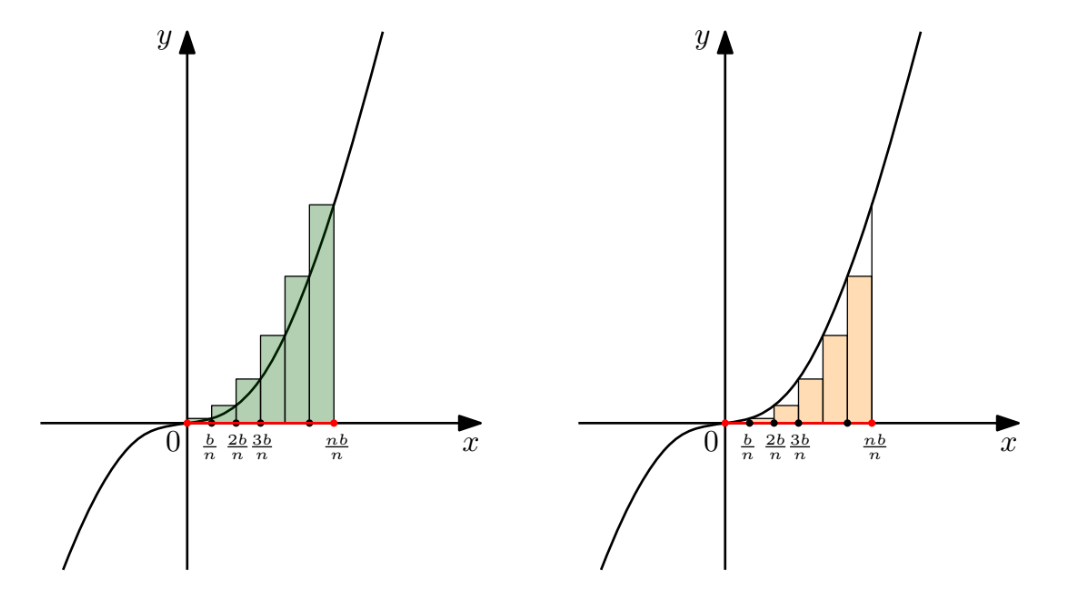
\includegraphics[width=0.7\textwidth]{img/lecture24/definite_integral}
		\end{center}
	\end{example}
	
	\begin{explanation}
	Площадь столбиков на левой картинке:
	\[ S_1 = \sum_{k = 1}^n \bigg(\frac{kb}{n}\bigg)^3 \frac{b}{n} = \sum_{k = 1}^n \frac{b^4}{n^4} \cdot k^3 = \frac{b^4}{n^4} \sum_{k = 1}^n k^3 = \frac{b^4}{n^4} (1 + 2 + ... + n)^2 (*) = \frac{b^4}{n^4} \frac{(n + 1)^2n^2}{4} \]
	
	(*) Формула суммы кубов доказывается по индукции.
	
	Площадь фигуры под графиком заведомо покрывается зелёными столбиками.
	
	Площадь столбиков на правой картинке:
	\[ S_2 = \sum_{k = 1}^n \bigg(\frac{(k - 1)b}{n}\bigg)^3 \frac{b}{n} = \sum_{k = 1}^n \frac{(k - 1)^3b^4}{n^4} \cdot k^3 = \frac{b^4}{n^4} \sum_{k = 1}^n (k - 1)^3 = \frac{b^4}{n^4} (1 + 2 + ... + n)^2 = \]
	\[ = \frac{b^4}{n^4} \frac{(n - 1)^2n^2}{4} \]
	
	Сумма $S_2$ меньше площади фигуры под графиком.
	\[ \lim_{n \to \infty} S_1 = \lim_{n \to \infty} \frac{b^4}{n^4} \frac{(n + 1)^2n^2}{4} = \lim_{n \to \infty} \frac{b^4}{4} \frac{(n + 1)^2}{n^2} = \lim_{n \to \infty} \frac{b^4}{4} \bigg(1 + \frac{1}{n}\bigg)^2 = \frac{b^4}{4} \]
	\[ \lim_{n \to \infty} S_2 = \lim_{n \to \infty} \frac{b^4}{n^4} \frac{(n - 1)^2n^2}{4} = \lim_{n \to \infty} \frac{b^4}{4} \frac{(n - 1)^2}{n^2} = \lim_{n \to \infty} \frac{b^4}{4} \bigg(1 - \frac{1}{n}\bigg)^2 = \frac{b^4}{4} \]
	
	По теореме о зажатой последовательности площадь фигуры равна $\frac{b^4}{4}$. Но можно было получить ответ, посчитав интеграл: $\displaystyle\int x^3 dx = \frac{x^4}{4} + C$.
	\end{explanation}
	
	\subsection{Интеграл Римана}
	
	\begin{definition}
		\begin{itemize}
			
			\item \underline{Разбиением} $T$ отрезка $[a, b]$ называется набор точек
			$a = x_0 < x_1 < ... < x_n = b$.
			
			\item Отрезки $[x_{k - 1}, x_k]$ называются \underline{отрезками разбиения}. Длину отрезка $[x_{k - 1}, x_k]$ обозначим через $\Delta x_k = x_k - x_{k - 1}, k \geqslant 1$.
			
			\item Величина $\Delta_T := \displaystyle \max_{1 \leqslant k \leqslant n} \Delta x_k$ называется \underline{диаметром разбиения}.
			
			\item \underline{Размеченным разбиением} $(T, \xi)$ отрезка $[a, b]$ называется пара, состоящая из разбиения $T$ отрезка $[a, b]$ и набора точек $\xi = (\xi_1, ..., \xi_n), \xi_k \in [x_{k - 1}, x_k]$.
			
			\item \underline{Интегральной суммой} функции $f$, соответствующей размеченному разбиению $(T, \xi)$, называется выражение
			\[ \sigma(f, T, \xi) := \sum^{n}_{k = 1} f(\xi_k) \Delta x_k. \]
		\end{itemize}
	\end{definition}
	
	\begin{definition}
		Функция $f$ называется интегрируемой по Риману на отрезке
		$[a, b]$, если существует такое число $I$, что $\forall \epsilon > 0 \exists \delta > 0: \forall$ размеченного разбиения $(T, \xi)$ с диаметром разбиения $\Delta_T < \delta$ выполнено $|\sigma(f, T, \xi) - I| < \epsilon$.
		
		Число $I$ называют интегралом функции $f$ на отрезке $[a, b]$ и
		обозначают $\displaystyle\int^{b}_{a} f(x) \; dx$.
	\end{definition}
	
	\begin{explanation}
		Геометрически мы уменьшаем длину отрезков и увеличиваем их число.
	\end{explanation}
	
	\begin{example}
		\begin{enumerate}
			\item $\displaystyle\int^{b}_{a} 1 \; dx = b - a$;
			\item Функция $I_{\Q}$ не интегрируема ни на каком отрезке.
		\end{enumerate}	
	\end{example}
	
	\begin{explanation}
		\begin{enumerate}
			\item $\sigma(f, T, \xi) = \sum^{n}_{k = 1} f(\xi_k) \Delta x_k = \sum^{n}_{k = 1} 1 \cdot \Delta x_k = \sum^{n}_{k = 1} \Delta x_k = b - a.$ (функция $f(\xi_k) = 1$ $\forall k$)
			
			\item Функция Дирихле $I_{\Q} : \R \rightarrow {0, 1}$ определяется следующим образом:
			\[\displaystyle I_{\Q} = \left\{{
				\begin{matrix}
					1, & x \in \Q \\
					0, & x \in \I
				\end{matrix}
			}\right.\]
			$\forall$ разбиения $T$ можно взять $\xi \in \Q$, $\zeta \in \I$ (внутри любого отрезка разбиения можно взять рациональное и иррациональное число)
			
			Тогда $\sigma(I_{\Q}, T, \xi) = \sum^{n}_{k = 1} I_{\Q}(\xi_k) \Delta x_k = \sum^{n}_{k = 1} 1 \cdot \Delta x_k = \sum^{n}_{k = 1} \Delta x_k = b - a$ и $\sigma(I_{\Q}, T, \zeta) = \sum^{n}_{k = 1} I_{\Q}(\zeta_k) \Delta x_k = \sum^{n}_{k = 1} 0 \cdot \Delta x_k = 0$.
			
			Тогда для любого $T$ с любым диаметром разбиения можно взять разметку, такую что иногда сумма равна $b - a$, иногда 1. Если $b - a \neq 0$, то функция не интегрируема.
		\end{enumerate}	
	\end{explanation}
	
	\newpage
    
    \section{Лекция 25: Интеграл Римана, суммы Дарбу}
    
    \begin{sentence}
    	Если функция $f$ интегрируема по Риману на отрезке $[a, b]$, то она ограничена на этом отрезке.
    \end{sentence}
    
    \begin{proof}
    	Пусть $f$ - интегрируема на $[a, b]$. 
    	
    	Тогда $\exists I \in \R : \forall \epsilon > 0$ $\exists \delta > 0$  $\forall (T, \xi)$ с $\Delta_T < \delta \rightarrow |\sigma(f, T, \xi) - I| < \epsilon \Leftrightarrow$ $\Leftrightarrow I - \epsilon < \sigma(f, T, \xi) < I + \epsilon$.
    	
    	$\sigma(f, T, \xi) = \sum^{n}_{k = 1} f(\xi_k) \Delta x_k.$
    	
    	Пусть $f$ - неограничена на $[a, b] \Rightarrow$ неограничена на одном из отрезков $\Delta_k,$ пусть на $\Delta_{k_0}$. Фиксируем $\xi_k$ для всех $k$ кроме $k_0$. Тогда $\sigma(f, T, \xi) = \sum^{n}_{k = 1} f(\xi_k) \Delta x_k = C + f(\xi_{k_0}) \Delta x_{k_0} \Rightarrow I - C - \epsilon < f(\xi_{k_0}) \Delta x_{k_0} < I - C + \epsilon \Rightarrow \frac{I - C - \epsilon}{\Delta x_{k_0}} < f(\xi_{k_0}) < \frac{I - C + \epsilon}{\Delta x_{k_0}}$ - противоречие, функция ограничена.
    \end{proof}
    
    \begin{sentence}[Линейность интеграла]
    	Пусть $f$ и $g$ интегрируемы по Риману на отрезке $[a, b]$. Тогда
    	для произвольных чисел $\alpha$, $\beta$ функция $\alpha f + \beta g$ интегрируема по Риману на отрезке $[a, b]$ и
    	\[ \displaystyle\int^b_a \alpha f(x) + \beta g(x) \; dx = \alpha \displaystyle\int^b_a f(x) \; dx + \beta \displaystyle\int^b_a g(x) \; dx. \]
    \end{sentence}
    
    \begin{proof}
    	$f$ - интегрируема на $[a, b] \Rightarrow \forall \epsilon > 0$ $\exists \delta_1 > 0 : \forall (T, \xi)$ с $\Delta_T < \delta_1 \rightarrow |\sigma(f, T, \xi) - I_1| < \epsilon.$ 
    	
    	$g$ - интегрируема на $[a, b] \Rightarrow \forall \epsilon > 0$ $\exists \delta_2 > 0 : \forall (T, \xi)$ с $\Delta_T < \delta_2 \rightarrow |\sigma(g, T, \xi) - I_2| < \epsilon.$
    	
    	Размеченное разбиение $(T, \xi)$ взяли одно и то же для обоих интегралов.
    	
    	Первые два утверждения означают, что $I_1 = \int_a^b f(x) \; dx, I_2 = \int_a^b g(x) \; dx.$
    	
    	Рассмотрим интегральную сумму 
    	\[ \sigma(\alpha f + \beta g, T, \xi) = \sum_{k = 1}^n (\alpha f(\xi_k) + \beta g(\xi_k)) \Delta x_k = \sum_{k = 1}^n \alpha f(\epsilon_k) \Delta x_k + \sum_{k = 1}^n \beta g(\xi_k) \Delta x_k = \]
    	\[ = \alpha \sigma(f, T, \xi) + \beta \sigma(g, T, \xi) \]
    	
    	Фиксируем $\epsilon > 0$ и возьмём $\delta = \min{(\delta_1, \delta_2)} \Rightarrow |\sigma(\alpha f + \beta g, T, \xi) - \alpha I_1 - \beta I_2| = |\alpha \sigma(f, T, \xi) + \beta \sigma(g, T, \xi) - \alpha I_1 - \beta I_2| \leqslant |\alpha \sigma(f, T, \xi) - \alpha I_1| + |\beta \sigma(g, T, \xi) - \beta I_2| \leqslant |\alpha| \epsilon + |\beta| \epsilon = (|\alpha| + |\beta|) \epsilon$
    	
    	$\forall \epsilon = \frac{\epsilon'}{2(|\alpha| + |\beta|)} > 0$ $\exists \delta = \min{(\delta_1, \delta_2)} > 0 : \forall (T, \xi)$ с $\Delta_T < \delta \rightarrow |\sigma(\alpha f + \beta g, T, \xi) - \alpha I_1 - \beta I_2| \leqslant (|\alpha| + |\beta|) \frac{\epsilon'}{2(|\alpha| + |\beta|)} = \frac{\epsilon'}{2} < \epsilon'.$ 
    \end{proof}
    
    \begin{sentence}[Монотонность интеграла]
    	Пусть $f$ и $g$ интегрируемы по Риману на отрезке $[a, b]$. Если
    	$f(x) \leqslant g(x)$ $\forall x \in [a, b],$ то $\displaystyle\int^b_a f(x) \; dx \leqslant \displaystyle\int^b_a g(x) \; dx.$
    \end{sentence}
    
    \begin{proof}
    	$f(x) \leqslant g(x) \Leftrightarrow g(x) - f(x) \geqslant 0$ и $\int_a^b f(x) \; dx \leqslant \int_a^b g(x) \; dx \Leftrightarrow \int_a^b g(x) - f(x) \; dx$ (пользуемся линейностью). Пусть $h(x) = g(x) - f(x) \Rightarrow$ требуется доказать, что $h(x) \geqslant 0 \Rightarrow \int_a^b h(x) \geqslant 0$.
    	
    	По определению $\forall \epsilon > 0$ $\exists \delta > 0 : \forall (T, \xi)$ c $\Delta_T < \delta \rightarrow  |\sigma(h, T, \xi) - \int_a^b h(x) \; dx| < \epsilon \Leftrightarrow \int_a^b h(x) - \epsilon < \underline{\sigma(h, T, \xi) < \int_a^b h(x) + \epsilon}$.
    	
    	$\sigma(h, T, \xi) \geqslant 0 (\text{т. к. } h(\xi_k) \geqslant 0 \Rightarrow \sum_{k = 1}^n h(\xi_k) \Delta x_k \geqslant 0) \Rightarrow \int_a^b h(x) + \epsilon > 0$ $\forall \epsilon > 0 \Rightarrow \int_a^b h(x) > -\epsilon$ $\forall \epsilon > 0 \Rightarrow \int_a^b h(x) \geqslant 0.$
    \end{proof}
    
    \begin{mention}
    	В частности, $\bigg|\displaystyle\int^b_a f(x) \; dx\bigg| \leqslant \displaystyle\int^b_a |f(x)| \; dx.$
    \end{mention}
    
    \begin{proof}
    	Далее мы докажем, что если $f(x)$ интегрируема, то и $|f(x)|$ интегрируема.
    	\[ -|f(x)| \leqslant f(x) \leqslant |f(x)|  \Rightarrow -\int_a^b |f(x)| \; dx \leqslant \int_a^b f(x) \; dx \leqslant \int_a^b |f(x)| \; dx \Rightarrow \]
    	\[ \Rightarrow \bigg| \int_a^b f(x) \; dx \bigg| \leqslant \int_a^b |f(x)| \; dx \]
    \end{proof}
    
    \subsection{Суммы и интегралы Дарбу}
    
    Фиксируем ограниченную функцию $f$, определённую на отрезке $[a, b]$.
    
    \begin{definition}
    	Для ограниченной на отрезке $[a, b]$ функции $f$ и разбиения $T$ определим \underline{нижнюю и верхнюю суммы Дарбу}:
    	\[s(f, T) := \sum^n_{k = 1}\inf_{x \in [x_{k - 1}, x_k]} f(x) \Delta x_k;\] (на каждом отрезке берём минимальное значение функции)
    	\[S(f, T) := \sum^n_{k = 1}\sup_{x \in [x_{k - 1}, x_k]} f(x) \Delta x_k.\] (на каждом отрезке берём максимальное значение функции)
    	
    	\underline{Нижним интегралом Дарбу} называется число $I_{*} = \displaystyle\sup_{T} s(f, T)$, а \underline{верхним ин-}
    	\underline{тегралом Дарбу} называется число $I^{*} = \displaystyle\inf_{T} S(f, T).$
    \end{definition}
    
    Сумма зелёных прямоугольников - это $s(f, T)$, сумма красных прямоугольников - это $S(f, T)$.
    
    \begin{center}
    	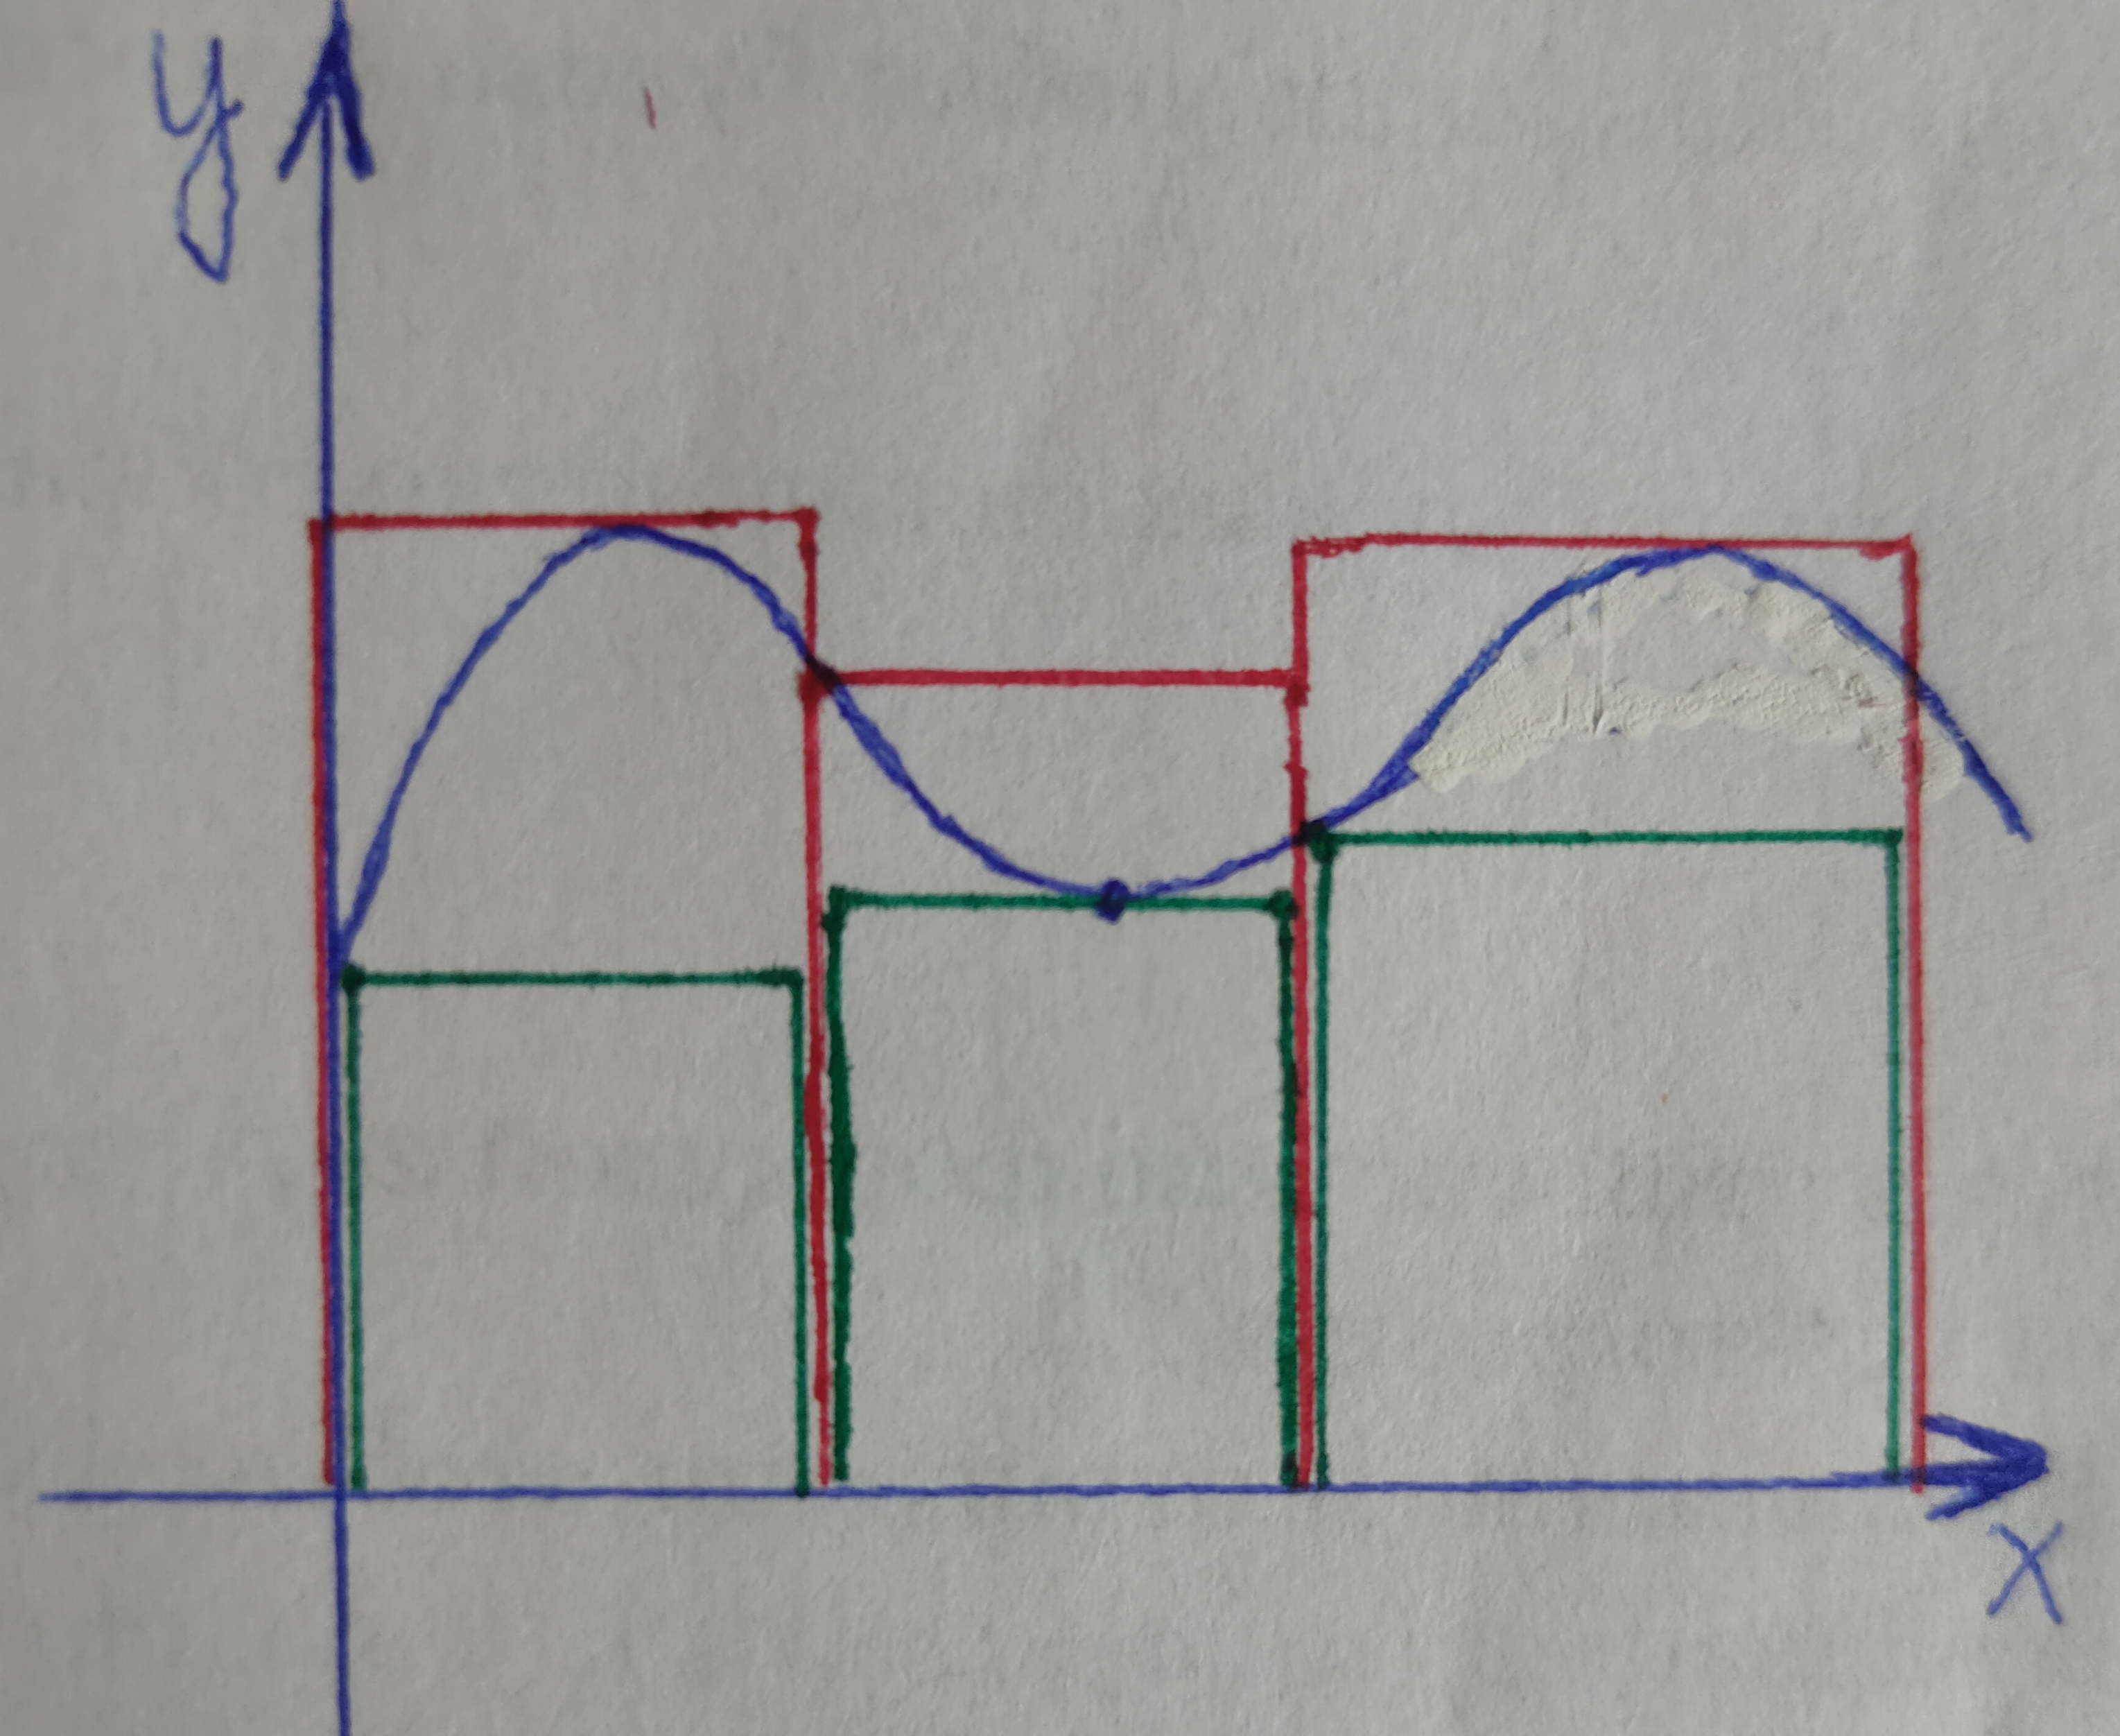
\includegraphics[width=0.4\textwidth]{img/lecture25/integral_darbu}
    \end{center}
    
    \subsection{Критерий Дарбу}
    
    \begin{lemma}
    	\begin{enumerate}
    		\item $s(f, T) \leqslant \displaystyle\inf_{\xi} \sigma(f, T, \xi) \leqslant \sigma(f, T, \xi) \leqslant \sup_{\xi}{\sigma(f, T, \xi)} \leqslant S(f, T);$
    		\item Если $T \subset T'$, то $s(f, T) \leqslant s(f, T')$ и $S(f, T') \leqslant S(f, T);$
    		\item $s(f, T_1) \leqslant s(f, T_1 \cup T_2) \leqslant S(f, T_1 \cup T_2) \leqslant S(f, T_2).$ 
    	\end{enumerate}
    \end{lemma}
    
    \begin{proof}
    	\begin{enumerate}
    		\item Докажем, что $\displaystyle s(f, T) = \inf_{\xi}{\sigma(f, T, \xi)}$
    		\begin{enumerate}
    			\item[$\leqslant$:] 
    			
    			$\forall \xi$ $\displaystyle s(f, T) = \sum_{k = 1}^n \inf_{\xi_k}{f(\xi_k) \Delta x_k} \leqslant \sum_{k = 1}^n f(\xi_k) \Delta x_k \Rightarrow s(f, T)$ - нижняя грань $\displaystyle \sum_{k = 1}^n f(\xi_k) \Delta x_k$.
    			
    			$\displaystyle \inf_{\xi}{\sum_{k = 1}^n f(\xi_k) \Delta x_k} = \inf_{\xi}{\sigma(f, T, \xi)}$ - точная нижняя грань $\Rightarrow \displaystyle s(f, T) \leqslant \inf_{\xi}{\sigma(f, T, \xi)}$.
    			
    			\item[$\geqslant$:] $\displaystyle s(f, T) = \sum_{k = 1}^n \inf_{\xi_k}{f(\xi_k) \Delta x_k}$
    			
    			По определенению инфимума $\forall \epsilon > 0$ $\displaystyle \exists \xi'_k \in \Delta_k : f(\xi'_k) \leqslant  \inf_{\xi_k}{f(\xi_k)} + \epsilon.$
    			
    			$\displaystyle \sigma(f, T, \xi') = \sum_{k = 1}^n f(\xi'_k) \Delta x_k \leqslant \sum_{k = 1}^n \bigg(\inf_{\xi_k}{f(\xi_k)} + \epsilon \bigg) \Delta x_k = s(f, T) + \epsilon(b - a)$
    			
    			$\displaystyle \inf_{\xi}{\sigma(f, T, \xi)} \leqslant \sigma(f, T, \xi') \leqslant s(f, T) + \epsilon(b - a)$
    			
    			При $\epsilon \to 0$, то $\displaystyle \inf_{\xi}{\sigma{(f, T, \xi)}} \leqslant s(f, T)$.
    		\end{enumerate}
    		Второе и третье неравенство в цепочке очевидное.
    		Четвёртое неравенство на самом деле является равенством и доказывается как первое равенство.
    		\item Рассмотрим отрезок $[a, b]$. На нём определено разбиение $T$. Теперь рассмотрим измельчение разбиения $T'$. Оно содержит те же точки, что и в $T$, но добавлет ещё свои точки.
    		
    		Красные точки - точки разбиения $T$, красные и синие точки - точки измельчения $T'$.
    		\begin{center}
    			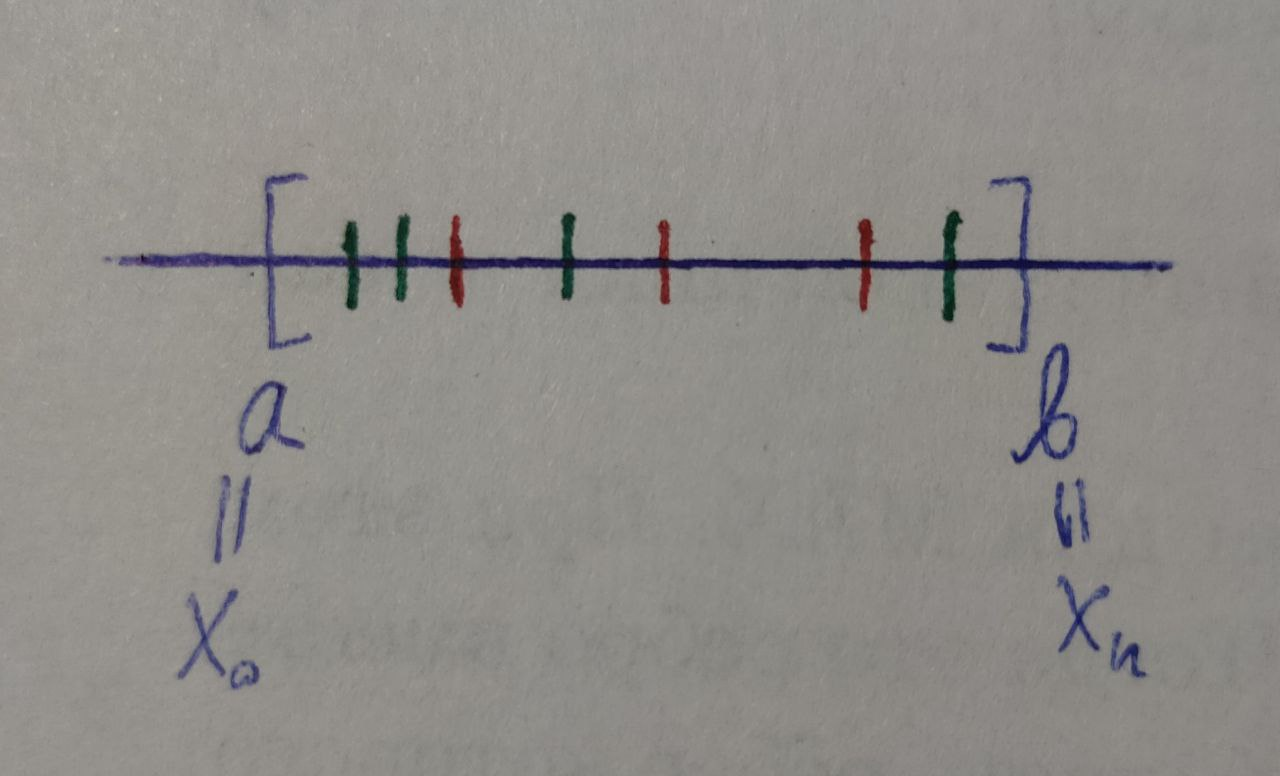
\includegraphics[width=0.3\textwidth]{img/lecture26/segment_division}
    		\end{center}
    		Пусть подотрезки $\Delta_k \in T$, а подотрезки $\Delta'_k \in T'$, $T \subset T'$. Рассмотрим отрезок $\Delta_k$ и будем считать, что он разбился на $k_j$ отрезков. Поэтому отрезок $\Delta'_k$ мы будем индексировать двумя индексами, первый номер - номер отрезка $\Delta_k$, в которым он лежит, второй номер - номер отрезка $\Delta'_k$ внутри отрезка $\Delta_k$.
    		\begin{center}
    			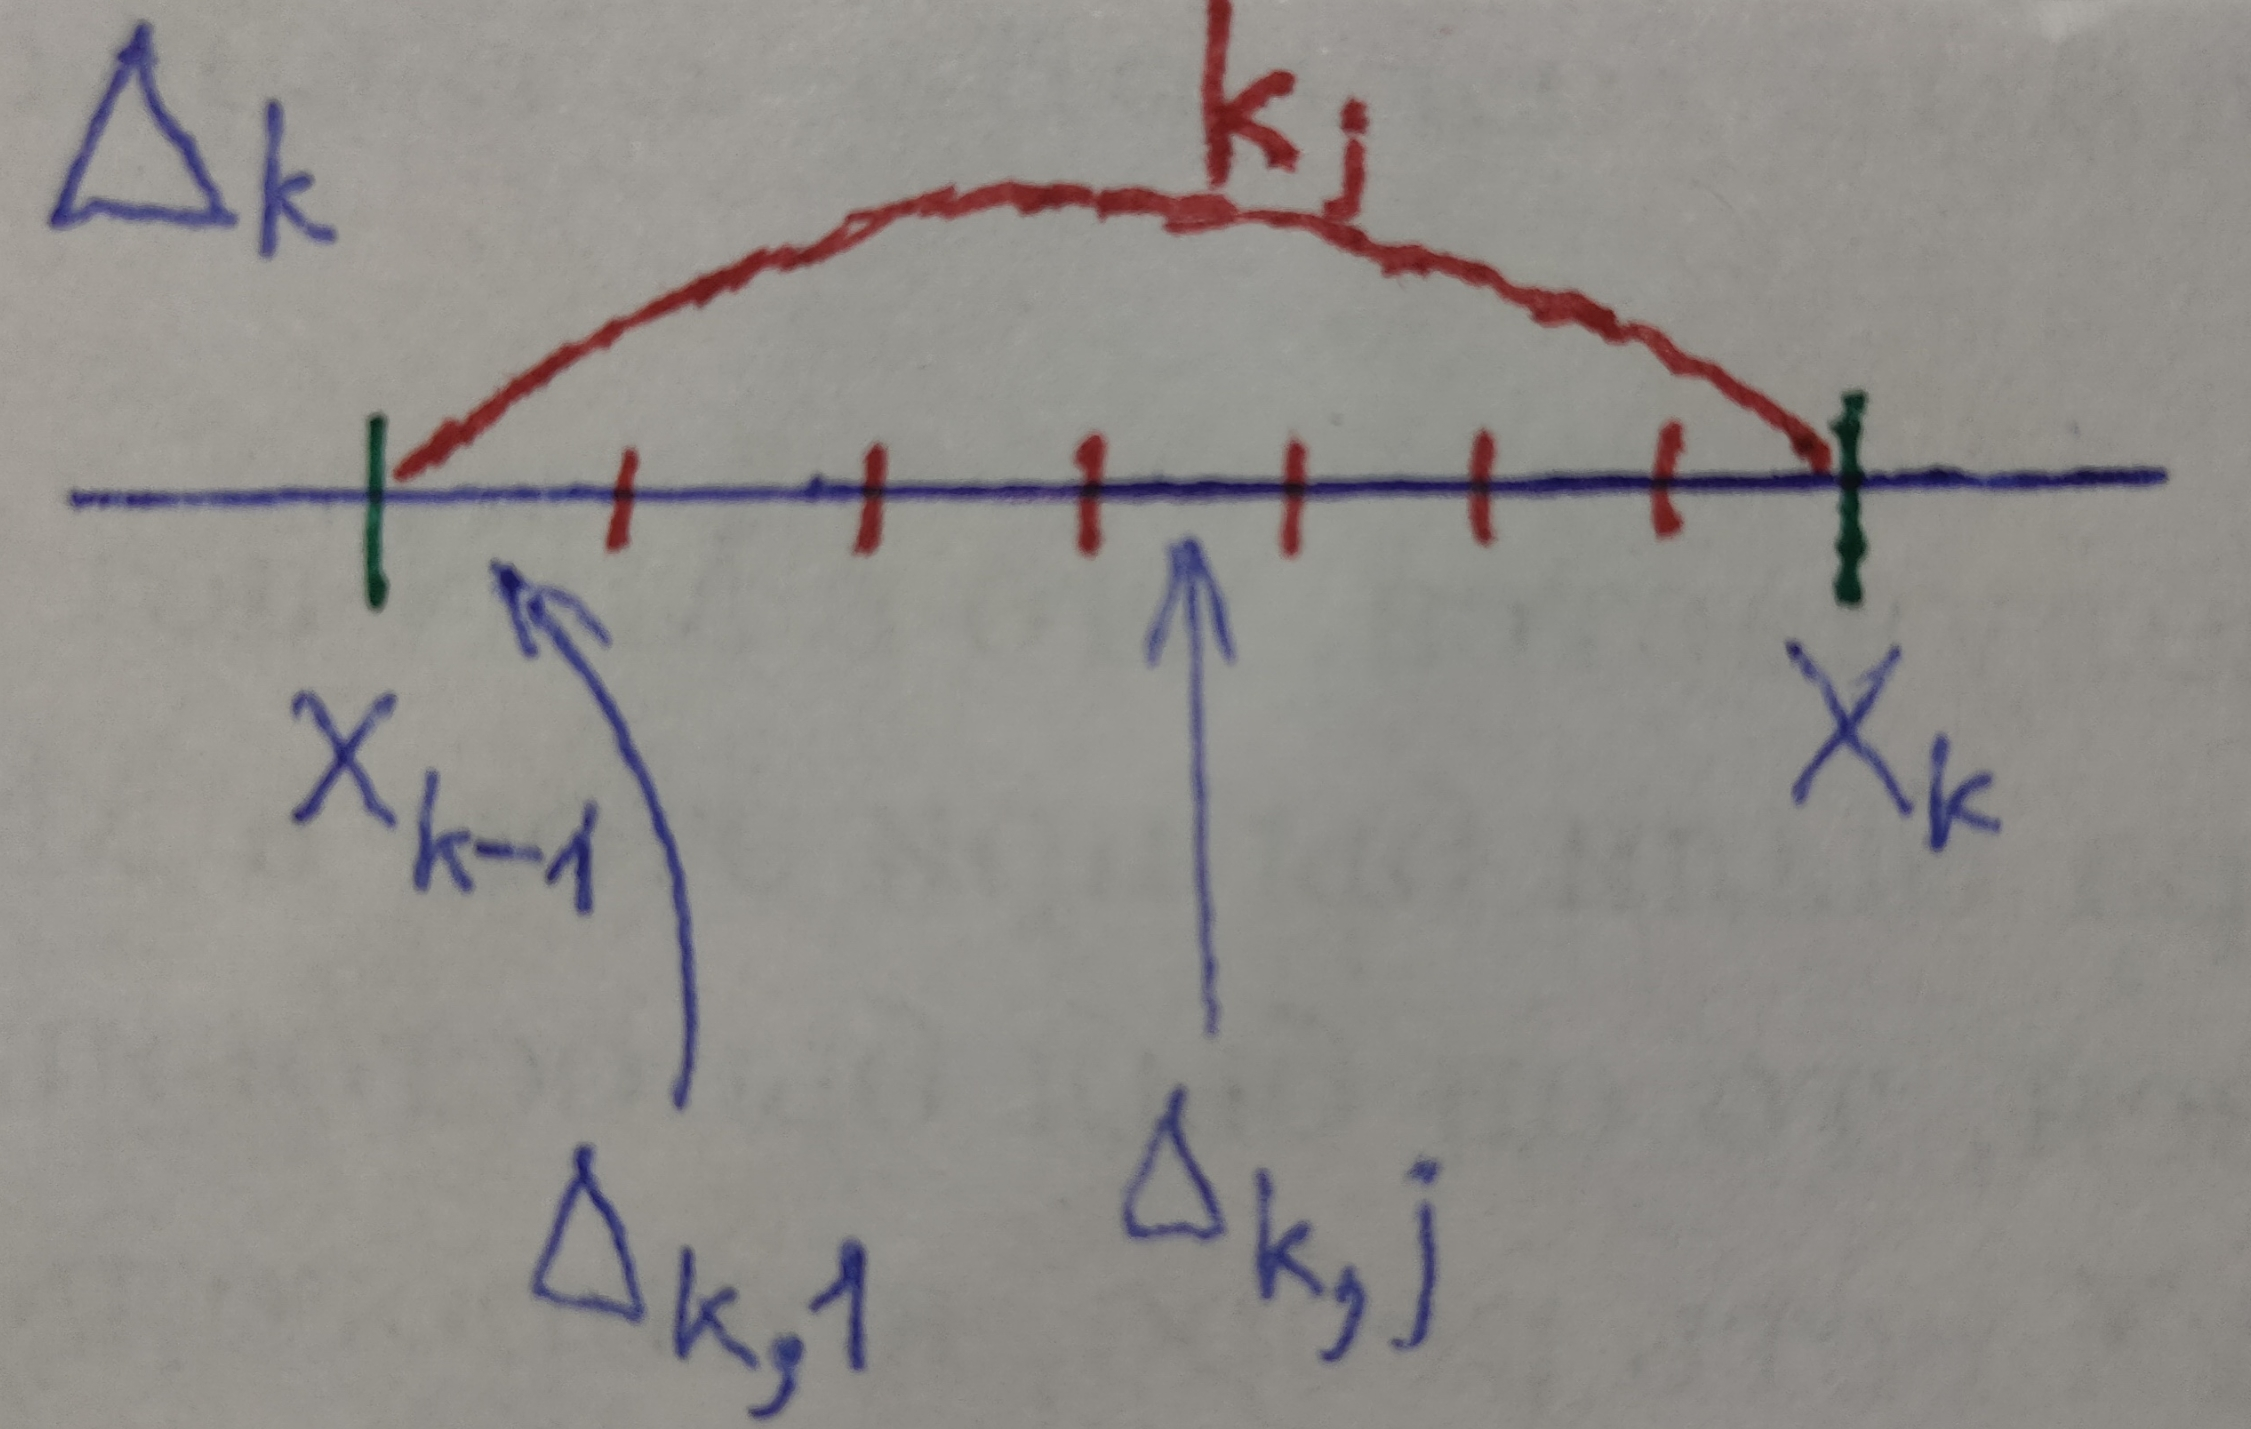
\includegraphics[width=0.3\textwidth]{img/lecture26/notations}
    		\end{center}
    		Тогда
    		\[ s(f, T') = \sum_{k = 1}^n\sum_{j = 1}^{k_j} \inf_{\xi \in \Delta_{k, j}}{f(\xi) \cdot \Delta x_{k, j}} \]
    		Приэтом на нескольких маленьких отрезках инфимум не меньше инфимума на одном большом отрезке, потому что на большом отрезке у нас есть больше точек, из которых мы можем выбрать меньшее значение. Если инфимум достигался на красном отрезке, то этот отрезок принадлежит большому, поэтому мы можем взять точку принадлежащую красному отрезку и получить инфимум на большом отрезке не больше, чем на маленьких. Поэтому
    		\[ s(f, T') = \sum_{k = 1}^n\sum_{j = 1}^{k_j} \inf_{\xi \in \Delta_{k, j}}{f(\xi) \cdot \Delta x_{k, j}} \geqslant \sum_{k = 1}^n\sum_{j = 1}^{k_j} \inf_{\xi \in \Delta_k}{f(\xi) \cdot \Delta x_{k, j}} \]
    		Продолжаем преобразования.
    		\[ \sum_{k = 1}^n \sum_{j = 1}^{k_j} \inf_{\xi \in \Delta_k}{f(\xi) \cdot \Delta x_{k, j}} = \sum_{k = 1}^n \inf_{\xi \in \Delta_k}{f(\xi) \sum_{j = 1}^{k_j} \Delta x_{k, j}} = \sum_{k = 1}^n \inf_{\xi \in \Delta_k}{f(\xi) \Delta x_k} = S(f, T) \]
    		Второе неравенство доказывается аналогично.
    		\item
    		\[ T_1 \subset T_1 \cup T_2 \Rightarrow \text{(из пункта 2) } s(f, T) \leqslant s(f, T_1 \cup T_2) \]
    		\[ \text{(из пункта 1) } s(f, T_1 \cup T_2) \leqslant S(f, T_1 \cup T_2) \]
    		\[ T_1 \cup T_2 \supset T_2 \Rightarrow \text{(из пункта 2) } S(f, T_1 \cup T_2) \leqslant S(f, T_2) \]
    	\end{enumerate}
    \end{proof}
    
    \newpage
    
    \section{Лекция 26: Интеграл Римана, суммы Дарбу}
    
    \begin{lemma}
    	$\forall \epsilon > 0$ $\exists \delta > 0:$ $\forall T$ с $\Delta_T < \delta$ выполнено $I_{*} \leqslant s(f, T) + \epsilon$ и $I^{*} \geqslant S(f, T) - \epsilon$.
    \end{lemma}
    
    \begin{proof}
    	По определению супремума
    	\[ I_{*} = \sup_T{s(f, T)} \Rightarrow \forall \epsilon > 0 \text{ } \exists T_{\epsilon} : I_{*} \leqslant s(f, T_{\epsilon}) + \epsilon \]
    	Рассмотрим произвольное разбиение $T$
    	\[ s(f, T_{\epsilon} \cup T) \geqslant \text{(пункт 2 предыдущей леммы)} s(f, T_{\epsilon}) \geqslant I_{*} - \epsilon \]
    	
    	Точки из разбиения $T$ окрасим в красный цвет, точки из $T_{\epsilon}$ - в чёрный цвет.
    	
    	\begin{center}
    		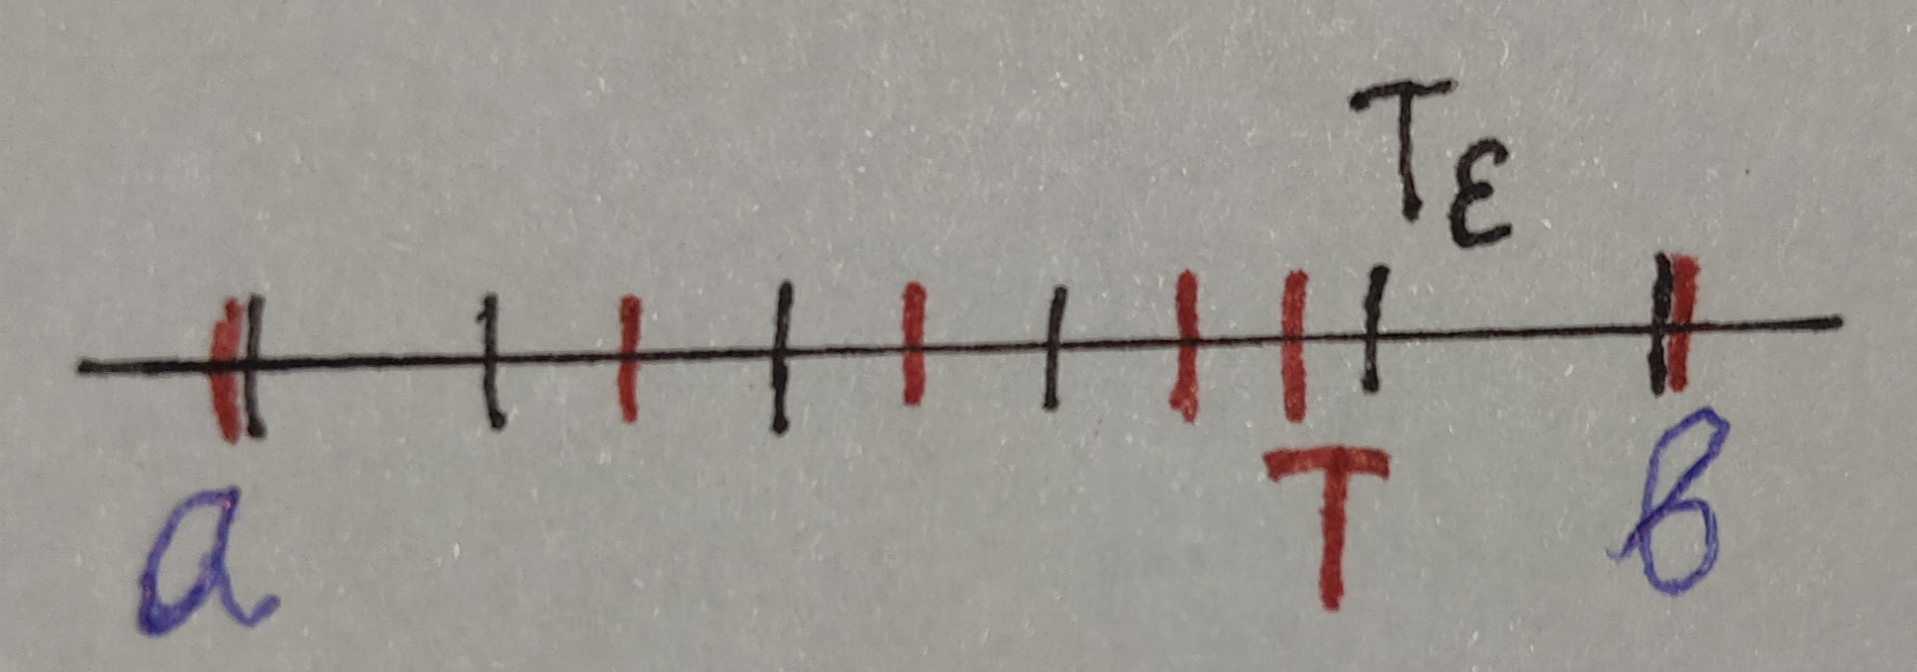
\includegraphics[width=0.2\textwidth]{img/lecture26/coloring_segments}
    	\end{center}
    	
    	Точки $T_{\epsilon}$ делят отрезок c чёрными концами на число чёрных точек + 1. Тогда (подразумеваем, что и в $T$, и в $T_{\epsilon}$ одинаковое число точек ????????) точки из $T_{\epsilon}$ могут разбить на не более, чем $2|T_{\epsilon}|$ отрезков, потому что максимум достигается, когда в каждом отрезке мы ставим по одной чёрной точке (т. е. разбиваем отрезок на два).
    	
    	\begin{center}
    		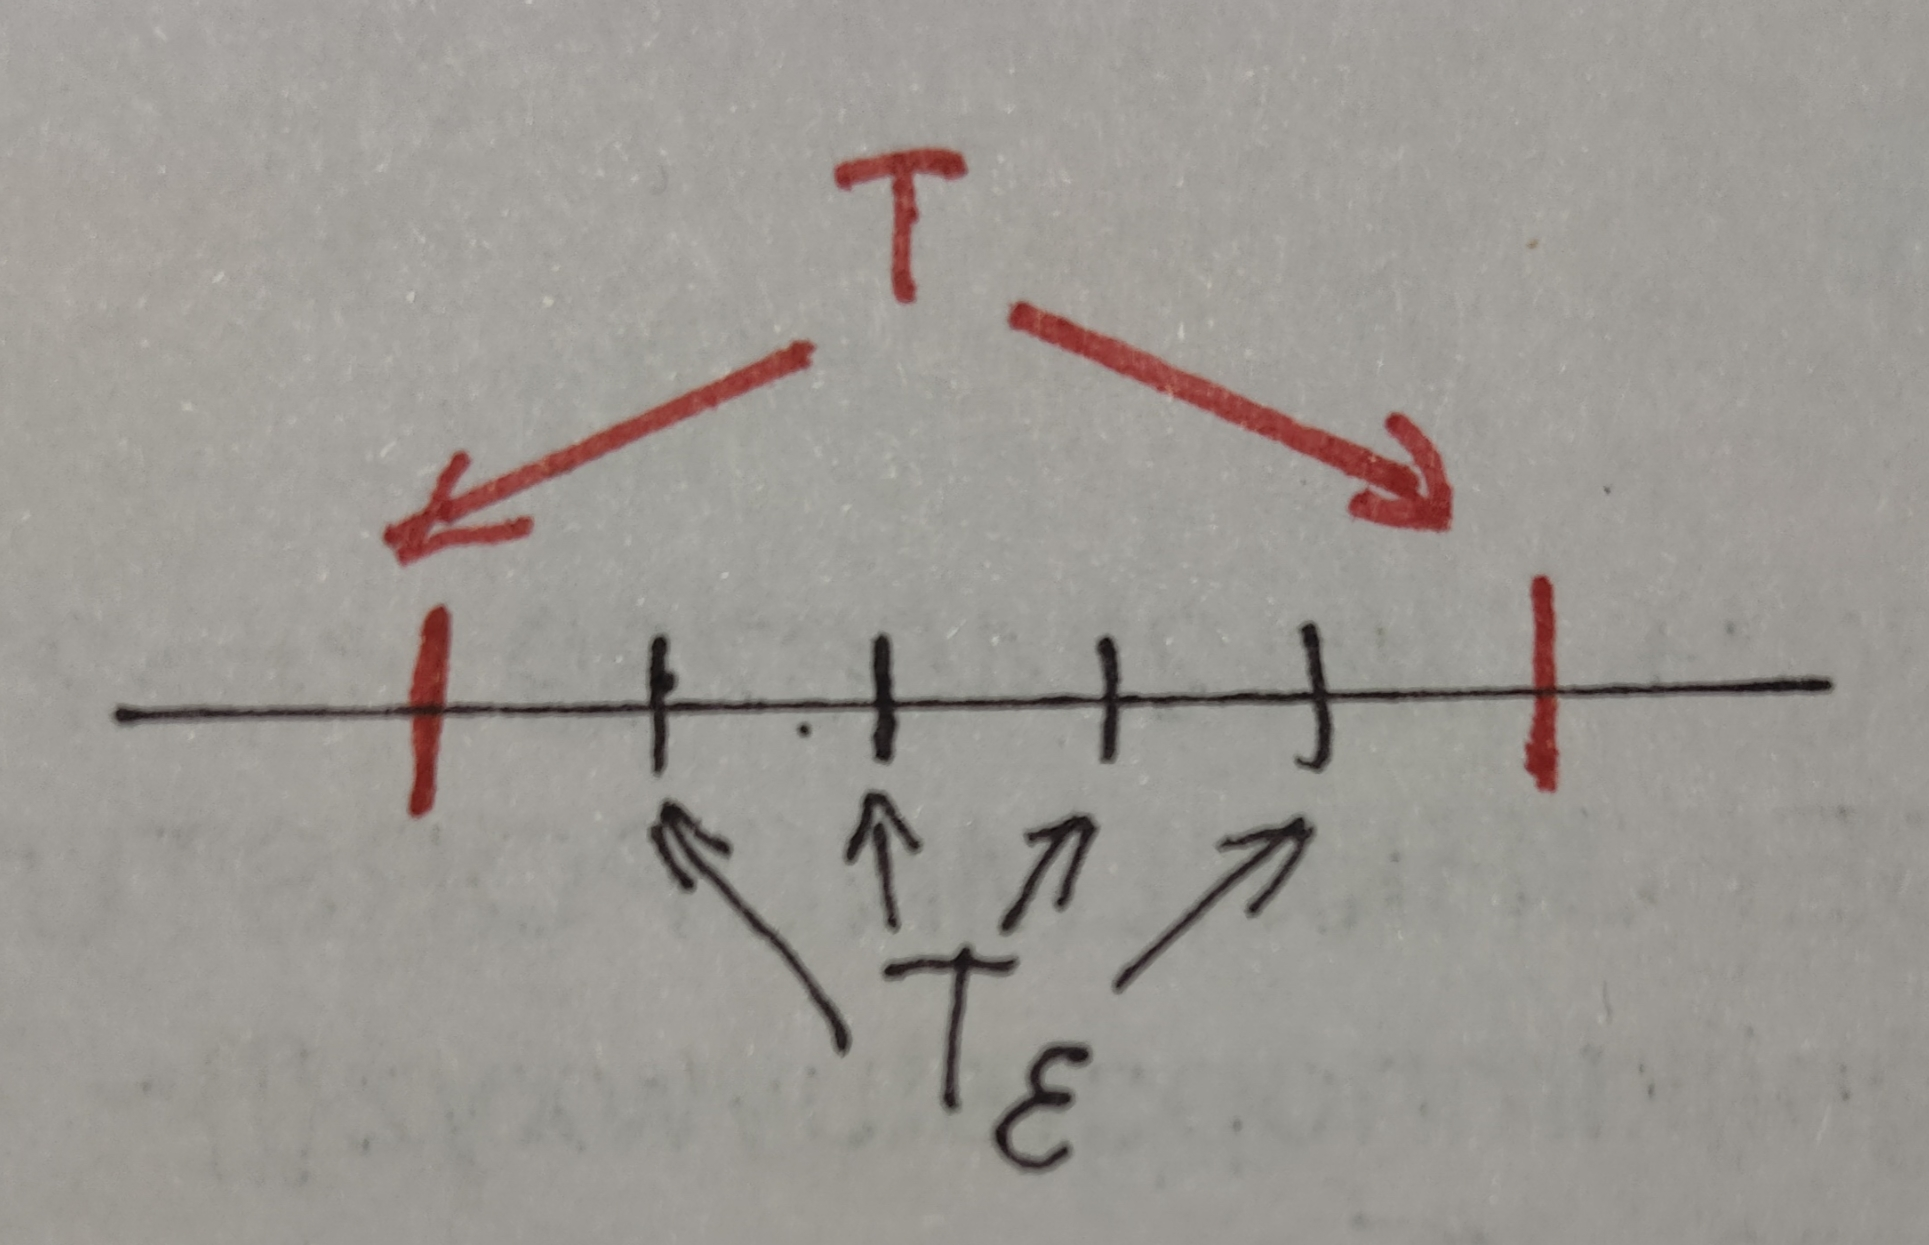
\includegraphics[width=0.2\textwidth]{img/lecture26/segment_number_estimation}
    	\end{center}
    	
    	\underline{Пояснение.} Здесь $\Delta_k$ - отрезок $[x_k, x_{k + 1}]$, подразумеваем под знаком суммы сумму по всем отрезкам, которые образуются этим множеством точек (отрезок образуют соседние точки, т. е. внутри отрезка других точек разбиения нет).
    	\[ s(f, T_{\epsilon} \cup T) = \sum_{\Delta_k \in T_{\epsilon} \cup T} \inf_{\xi \in \Delta_k} {f(\xi) \cdot \Delta x_k} = \sum_{\Delta_k \in T_{\epsilon} \cup T \text{ и } \Delta_k \in T} \inf_{\xi \in \Delta_k} {f(\xi) \cdot \Delta x_k} + \]
    	\[ + \sum_{\Delta_k \in T_{\epsilon} \cup T \text{ и } \Delta_k \not\in T} \inf_{\xi \in \Delta_k} {f(\xi) \cdot \Delta x_k} = (*) \]
    	Первая сумма - сумма отрезков с красными концами, вторая сумма - сумма остальных отрезков (т. е. либо оба конца чёрные, либо один конец чёрный, а другой - красный).
    	Первое слагаемое выразим как разность суммы по всем отрезкам с красными концами и суммы по всем отрезкам с красными концами, но с чёрными точками внутри.
    	\[ (*) = \sum_{\Delta_k \in T} \inf_{\xi \in \Delta_k} {f(\xi) \Delta x_k} - \sum_{\Delta_k \in T \text{ и } \Delta_k \not\in T \cup T_{\epsilon}} {\inf_{\xi \in \Delta_k} {f(\xi) \cdot \Delta x_k}} + \sum_{\Delta_k \in T_{\epsilon} \cup T \text{ и } \Delta_k \not\in T} {\inf_{\xi \in \Delta_k} {f(\xi) \cdot \Delta x_k}} \leqslant \]
    	\[ \leqslant s(f, T) + 2\sup_{x \in [a, b]} {|f(x)| \cdot \Delta_T \cdot 2|T_{\epsilon}|} \]
    	В конце - грубая оценка для последних двух слагаемых.
    	
    	Возьмём $\displaystyle \delta = \frac{\epsilon}{\displaystyle2\sup_{x \in [a, b]} {|f(x)| \cdot 2|T_{\epsilon}|}}$. Тогда для $T$ c $\Delta_T < \delta$
    	\[ I_{*} \leqslant s(f, T_{\epsilon}) + \epsilon \leqslant s(f, T \cup T_{\epsilon}) + \epsilon \leqslant s(f, T) + 2\sup_{x \in [a, b]} {|f(x)| \cdot \Delta_T \cdot 2|T_{\epsilon}|} + \epsilon < \]
    	\[ < s(f, T) + 2\sup_{x \in [a, b]} {|f(x)| \cdot \delta \cdot 2|T_{\epsilon}|} + \epsilon = s(f, T) + \epsilon + \epsilon = s(f, T) + 2\epsilon \]
    	
    	Заменой $\epsilon = \frac{\epsilon'}{2}$ получаем $I_{*} \leqslant s(f, T) + \epsilon'$.
    	
    	Аналогично доказывается, что $I^{*} \geqslant S(f, T) - \epsilon$.
    	
    	\underline{Уточнение.} Если фиксируем $\epsilon$, то $T_{\epsilon}$ - фиксированное число. $f(x)$ интегрируема $\Rightarrow$ она ограничена (по предложению 25.1) $\Rightarrow$ супремум ограничен, поэтому такое $\delta$ рассматривать корректно.
    \end{proof}
    
    \begin{theorem}[Критерий Дарбу]
    	Ограниченная функция $f$ интегрируема по Риману на отрезке $[a, b]$ тогда и только тогда, когда $I^{*} = I_{*}$.
    \end{theorem}
    
    \begin{proof}
    	\begin{enumerate}
    		\item[$\Rightarrow$] Если функция интегрируема, то 
    		\[ \forall \epsilon > 0 \text{ } \exists \delta > 0: \forall (T, \xi) \text{ с } \Delta_T < \delta \rightarrow |\sigma(f, T, \xi) - I| < \epsilon \]
    		\[ I - \epsilon < \sigma(f, T, \xi) < I + \epsilon \]
    		\[ I - \epsilon \leqslant \inf_{\xi} {\sigma(f, T, \xi)} = s(f, T) \leqslant \sup_{T} {s(f, T)} = I_{*} \]
    		\[ I^{*} = \inf_{T} {S(f, T)} \leqslant S(f, T) = \sup_{\epsilon} {\sigma(f, T, \xi)} \leqslant I + \epsilon \]
    		
    		Докажем, что $I_{*} \leqslant I^{*}$:
    		\[ \forall T_1, T_2 \text{ } s(f, T_1) \leqslant S(f, T_2) \Rightarrow \sup_{T_1} {s(f, T_1)} \leqslant S(f, T_2) \Rightarrow \sup_{T_1} {s(f, T_1)} \leqslant S(f, T_2) \Rightarrow \]
    		\[ \Rightarrow \sup_{T_1} {s(f, T_1)} \leqslant \inf_{T_2} {S(f, T_2)} \]
    		Тогда
    		\[ I - \epsilon \leqslant I_{*} \leqslant I^{*} \leqslant I + \epsilon \]
    		Устремляя $\epsilon \to 0$, получаем, что $I_{*} = I^{*}$.
    		\item[$\Leftarrow$] $I = I_{*} = I^{*}$
    		\[ \forall \epsilon > 0 \text{ } \exists \delta > 0 : \forall T \text{ с } \Delta_T < \delta \rightarrow I - \epsilon = I_{*} - \epsilon \leqslant (\text{лемма 26.1}) \text{ } s(f, T) \leqslant \]
    		\[ \leqslant \sigma(f, T, \xi) \leqslant S(f, T) \leqslant (\text{лемма 26.1}) \text{ } I^{*} + \epsilon = I + \epsilon \Rightarrow |\sigma(f, T, \xi) - I| < \epsilon, \]
    		что есть определение интеграла.
    	\end{enumerate}
    \end{proof}
    
    \subsection{Колебание функции}
    
    \begin{definition}
    	\underline{Колебанием} функции $f$ на отрезке $\Delta$ называется число
    	\[ \omega(f, \Delta) := \sup_{x, y \in \Delta}{|f(x) - f(y)|} = \sup_{x \in \Delta}{f(x)} - \inf_{y \in \Delta}{f(y)}. \]
    \end{definition}
    
    \begin{explanation}
    	\begin{enumerate}
    		\item В одну сторону
    		\[ \forall x, y \in \Delta \text{ } f(x) - f(y) \leqslant \sup_{x, y \in \Delta} {(f(x))} - f(y) \leqslant \sup_{x \in \Delta} {f(x)} - \inf_{y \in \Delta} {f(y)} \Rightarrow \]
    		\[ \Rightarrow \sup_{x, y \in \Delta}{|f(x) - f(y)|} \leqslant \sup_{x \in \Delta}{f(x)} - \inf_{y \in \Delta}{f(y)} \] 
    		\item В другому сторону
    		
    		По определению супремума и инфимума
    		\[ \forall \delta > 0 \text{ } \exists x_{\delta}: \sup_{x \in \Delta} {f(x)} \leqslant f(x_{\delta}) + \delta \]
    		\[ \forall \delta > 0 \text{ } \exists y_{\delta}: \sup_{y \in \Delta} {f(y)} \geqslant f(y_{\delta}) + \delta \]
    		Тогда
    		\[ \sup_{x \in \Delta} {f(x)} - \inf_{y \in \Delta}{f(y)} \leqslant f(x_{\delta}) - f(y_{\delta}) + 2\delta \leqslant  \sup_{x, y \in \Delta} {|f(x) - f(y)|} + 2\delta \Rightarrow \]
    		\[ \Rightarrow \sup_{x \in \Delta} {f(x)} - \inf_{y \in \Delta}{f(y)} \leqslant  \sup_{x, y \in \Delta} {|f(x) - f(y)|} \text{ при } \delta \to 0 \]
    	\end{enumerate}
    \end{explanation}
    
    \newpage
    
    \section{Лекция 27: Интегрируемость по Риману различных классов функций}
    
    \begin{theorem}
    	Пусть $f$ - ограниченная на отрезке $[a, b]$ функция. Тогда следующие условия эквивалентны:
    	\begin{enumerate}
    		\item $I^{*} = I_{*}$;
    		\item Функция $f$ интегрируема на $[a, b]$;
    		\item $\forall \epsilon > 0$ $\exists \delta > 0: \forall T$ с $\Delta_T < \delta:$
    		\[ \sum_{k = 1}^{n} \omega(f, \Delta_k) \Delta x_k < \epsilon; \]
    		\item $\forall \epsilon > 0$ $\exists T:$
    		\[ \sum_{k = 1}^{n} \omega(f, \Delta_k) \Delta x_k < \epsilon; \]
    	\end{enumerate}
    \end{theorem}
    
    \begin{proof}
    	Заметим, что
    	\[ S(f, T) - s(f, T) = \sum_{k = 1}^n \sup_{\xi \in \Delta_k} f(\xi) \Delta x_k - \sum_{k = 1}^n \inf_{\xi \in \Delta_k} f(\xi) \Delta x_k = \]
    	\[ = \sum_{k = 1}^n \bigg(\sup_{\xi \in \Delta_k} f(\xi) \Delta x_k - \inf_{\xi \in \Delta_k} f(\xi) \Delta x_k\bigg) = \sum_{k = 1}^n \omega(f, \Delta_k) \Delta x_k \]
    	
    	\begin{enumerate}
    		\item[$1 \Rightarrow 2$] Применяем критерий Дарбу.
    		\item[$2 \Rightarrow 3$] Пусть $f$ - интегрируемая функция на $[a, b]$. Тогда $I^{*} = I_{*} = I$.
    		
    		По лемме 26.1
    		\[ \forall \epsilon > 0 \text{ } \exists \delta > 0: \forall T \text{ c } \Delta_T < \delta:
    		\displaystyle \left\{{
    			\begin{matrix}
    				I = I^{*} \geqslant S(f, T) - \epsilon, \\
    				I = I_{*} \leqslant s(f, T) + \epsilon. \\
    			\end{matrix}
    		}\right. \Rightarrow \]
    		\[ \Rightarrow I - I \leqslant s(f, T) - S(f, T) + 2\epsilon \]
    		По замечанию заключаем
    		\[ \sum_{k = 1}^n \omega(f, \Delta_k) \Delta x_k \leqslant 2\epsilon \]
    		\item[$3 \Rightarrow 4$] По предыдущему пункту существует такое $T$ с диаметром $\Delta_T < \delta$, значит и просто $T$ существует.
    		\item[$4 \Rightarrow 1$] В доказательстве критерия Дарбу мы получили следующую цепочку неравенств
    	    \[ s(f, T) \leqslant I_{*} \leqslant I^{*} \leqslant S(f, T) \]
    	    Тогда
    	    \[ 0 \leqslant I^{*} - I_{*} \leqslant S(f, T) - s(f, T) \leqslant \sum_{k = 1}^n \omega(f, \Delta_k) \Delta x_k < \epsilon \Rightarrow \text{ при } \epsilon \to 0 \text{ } I^{*} = I_{*} \]
    	\end{enumerate}
    \end{proof}
    
     \subsection{Интегрируемость модуля, квадрата и произведения функций}
    
    \begin{corollary}
    	Если $f$ интегрируема по Риману на отрезке $[a, b]$, то $|f|$ и $f^2$ интегрируемы по Риману на отрезке $[a, b]$ и для любого $[c, d] \subset [a, b]$ функция $f$ интегрируема по Риману на отрезке
    	$[c, d]$.
    \end{corollary}
    
    \begin{proof}
    	$f$ - интегрируема на $[a, b] \Leftrightarrow$ по пункту 4 теоремы 27.1 
    	\[ \forall \epsilon > 0 \text{ } \exists T: \sum_{k = 1}^n \omega(f, \Delta_k) \Delta x_k < \epsilon. \]
    	\underline{Доказательство для модуля функции}
    	
    	(Неравенство треугольника: $|A| - |B| \leqslant |A - B|, |B| - |A| \leqslant |A - B| \Rightarrow ||A| - |B|| \leqslant |A - B|$)
    	\[ \omega(|f|, \Delta_k) = \sup_{x, y \in \Delta_k} {||f(x)| - |f(y)||} \leqslant \sup_{x, y \in \Delta_k} {|f(x) - f(y)|} = \omega(f, \Delta_k) \Rightarrow \]
    	\[ \Rightarrow 0 \leqslant \sum_{k = 1}^n {\omega(|f|, \Delta_k)} \Delta x_k \leqslant \sum_{k = 1}^n \omega(f, \Delta_k) \Delta x_k < \epsilon \]
    	\underline{Доказательство для квадрата функции}
    	\[ \omega(f^2, \Delta_k) = \sup_{x, y \in \Delta_k} {|f^2(x) - f^2(y)|} = \sup_{x, y \in \Delta_k} {|(f(x) - f(y))(f(x) + f(y))|} \leqslant \]
    	\[ \leqslant \sup_{x, y \in \Delta_k} {|f(x) - f(y)|(|f(x)| + |f(y)|)} \leqslant 2\sup_{x \in \Delta_k} {|f(x)|} \sup_{x, y \in \Delta_k} {|f(x) - f(y)|} = \]
    	\[ = 2\sup_{x \in \Delta_k} {|f(x)|} \cdot \omega(f, \Delta_k) \]
    	\[ \sum_{k = 1}^n \omega(f^2, \Delta_k) \Delta x_k \leqslant \sum_{k = 1}^n 2\sup_{x \in \Delta_k} {|f(x)| \omega(f, \Delta_k) \Delta x_k} \leqslant 2\sup_{x \in [a, b]} |f(x)| \sum_{k = 1}^n \omega(f, \Delta_k) \Delta x_k \leqslant \]
    	\[ \leqslant M \cdot \epsilon, \text{где M - константа}. \]
    	
    	В обоих случаях в конце мы применяем теорему 27.1 и заключаем, что функции интегрируемы на $[a, b]$.
    	
    	Интегрируемость функции на подотрезке докажем далее.
    \end{proof}
    
    \begin{corollary}
    	Если $f$ и $g$ интегрируемы на $[a, b]$, то и $f \cdot g$ интегрируема на $[a, b]$.
    \end{corollary}
    
    \begin{proof}
    	Если $f$ и $g$ интегрируемы, то $f - g$ и $f + g$ интегрируемы. Тогда их квадраты $(f - g)^2$ и $(f + g)^2$ интегрируемы. Следовательно, $\frac{1}{4}((f + g)^2 - (f - g)^2) = \frac{1}{4} \cdot 4fg = fg$ интегрируема.
    \end{proof}
    
    \subsection{Интегрируемость монотонной функции}
    
    \begin{corollary}
    	Если $f$ монотонна на $[a, b]$, то $f$ интегрируема по Риману на $[a, b]$.
    \end{corollary}
    
    \begin{proof}
    	Без ограничения общности пусть $f$ - возрастающая функция.
    	\[ \omega(f, \Delta_k) = f(x_k) - f(x_{k - 1}) \]
    	\[ \sum_{k = 1}^n \omega(f, \Delta_k) \cdot \Delta x_k = \sum_{k = 1}^n (f(x_k) - f(x_{k - 1})) \Delta x_k = (*) \]
    	Пусть $\Delta x_k = \Delta x_j$ $\forall k, j$. Тогда
    	\[ (*) = \Delta x_1 \sum_{k = 1}^n (f(x_k) - f(x_{k - 1})) = \Delta_T (f(b) - f(a)) \]
    	Следовательно, $\forall T -$ разбиение $[a, b]$ на одинаковые части с $\Delta_T < \frac{\epsilon}{f(b) - f(a)}$
    	\[ \sum_{k = 1}^n \omega(f, \Delta_k) \Delta x_k \leqslant \epsilon \cdot (f(b) - f(a)). \]
    	
        Для убывающей $f$ доказывается аналогично.
    \end{proof}
    
    \subsection{Равномерная непрерывность}
    
    \begin{definition}
    	\item Функция $f$ называется \underline{равномерно непрерывной} на
    	множестве $X$, если $\forall \epsilon > 0$ $\exists \delta > 0$ для которого из неравенства
    	$|x - y| < \delta$ следует $|f(x) - f(y)| < \epsilon.$
    \end{definition}
    
    \begin{center}
    	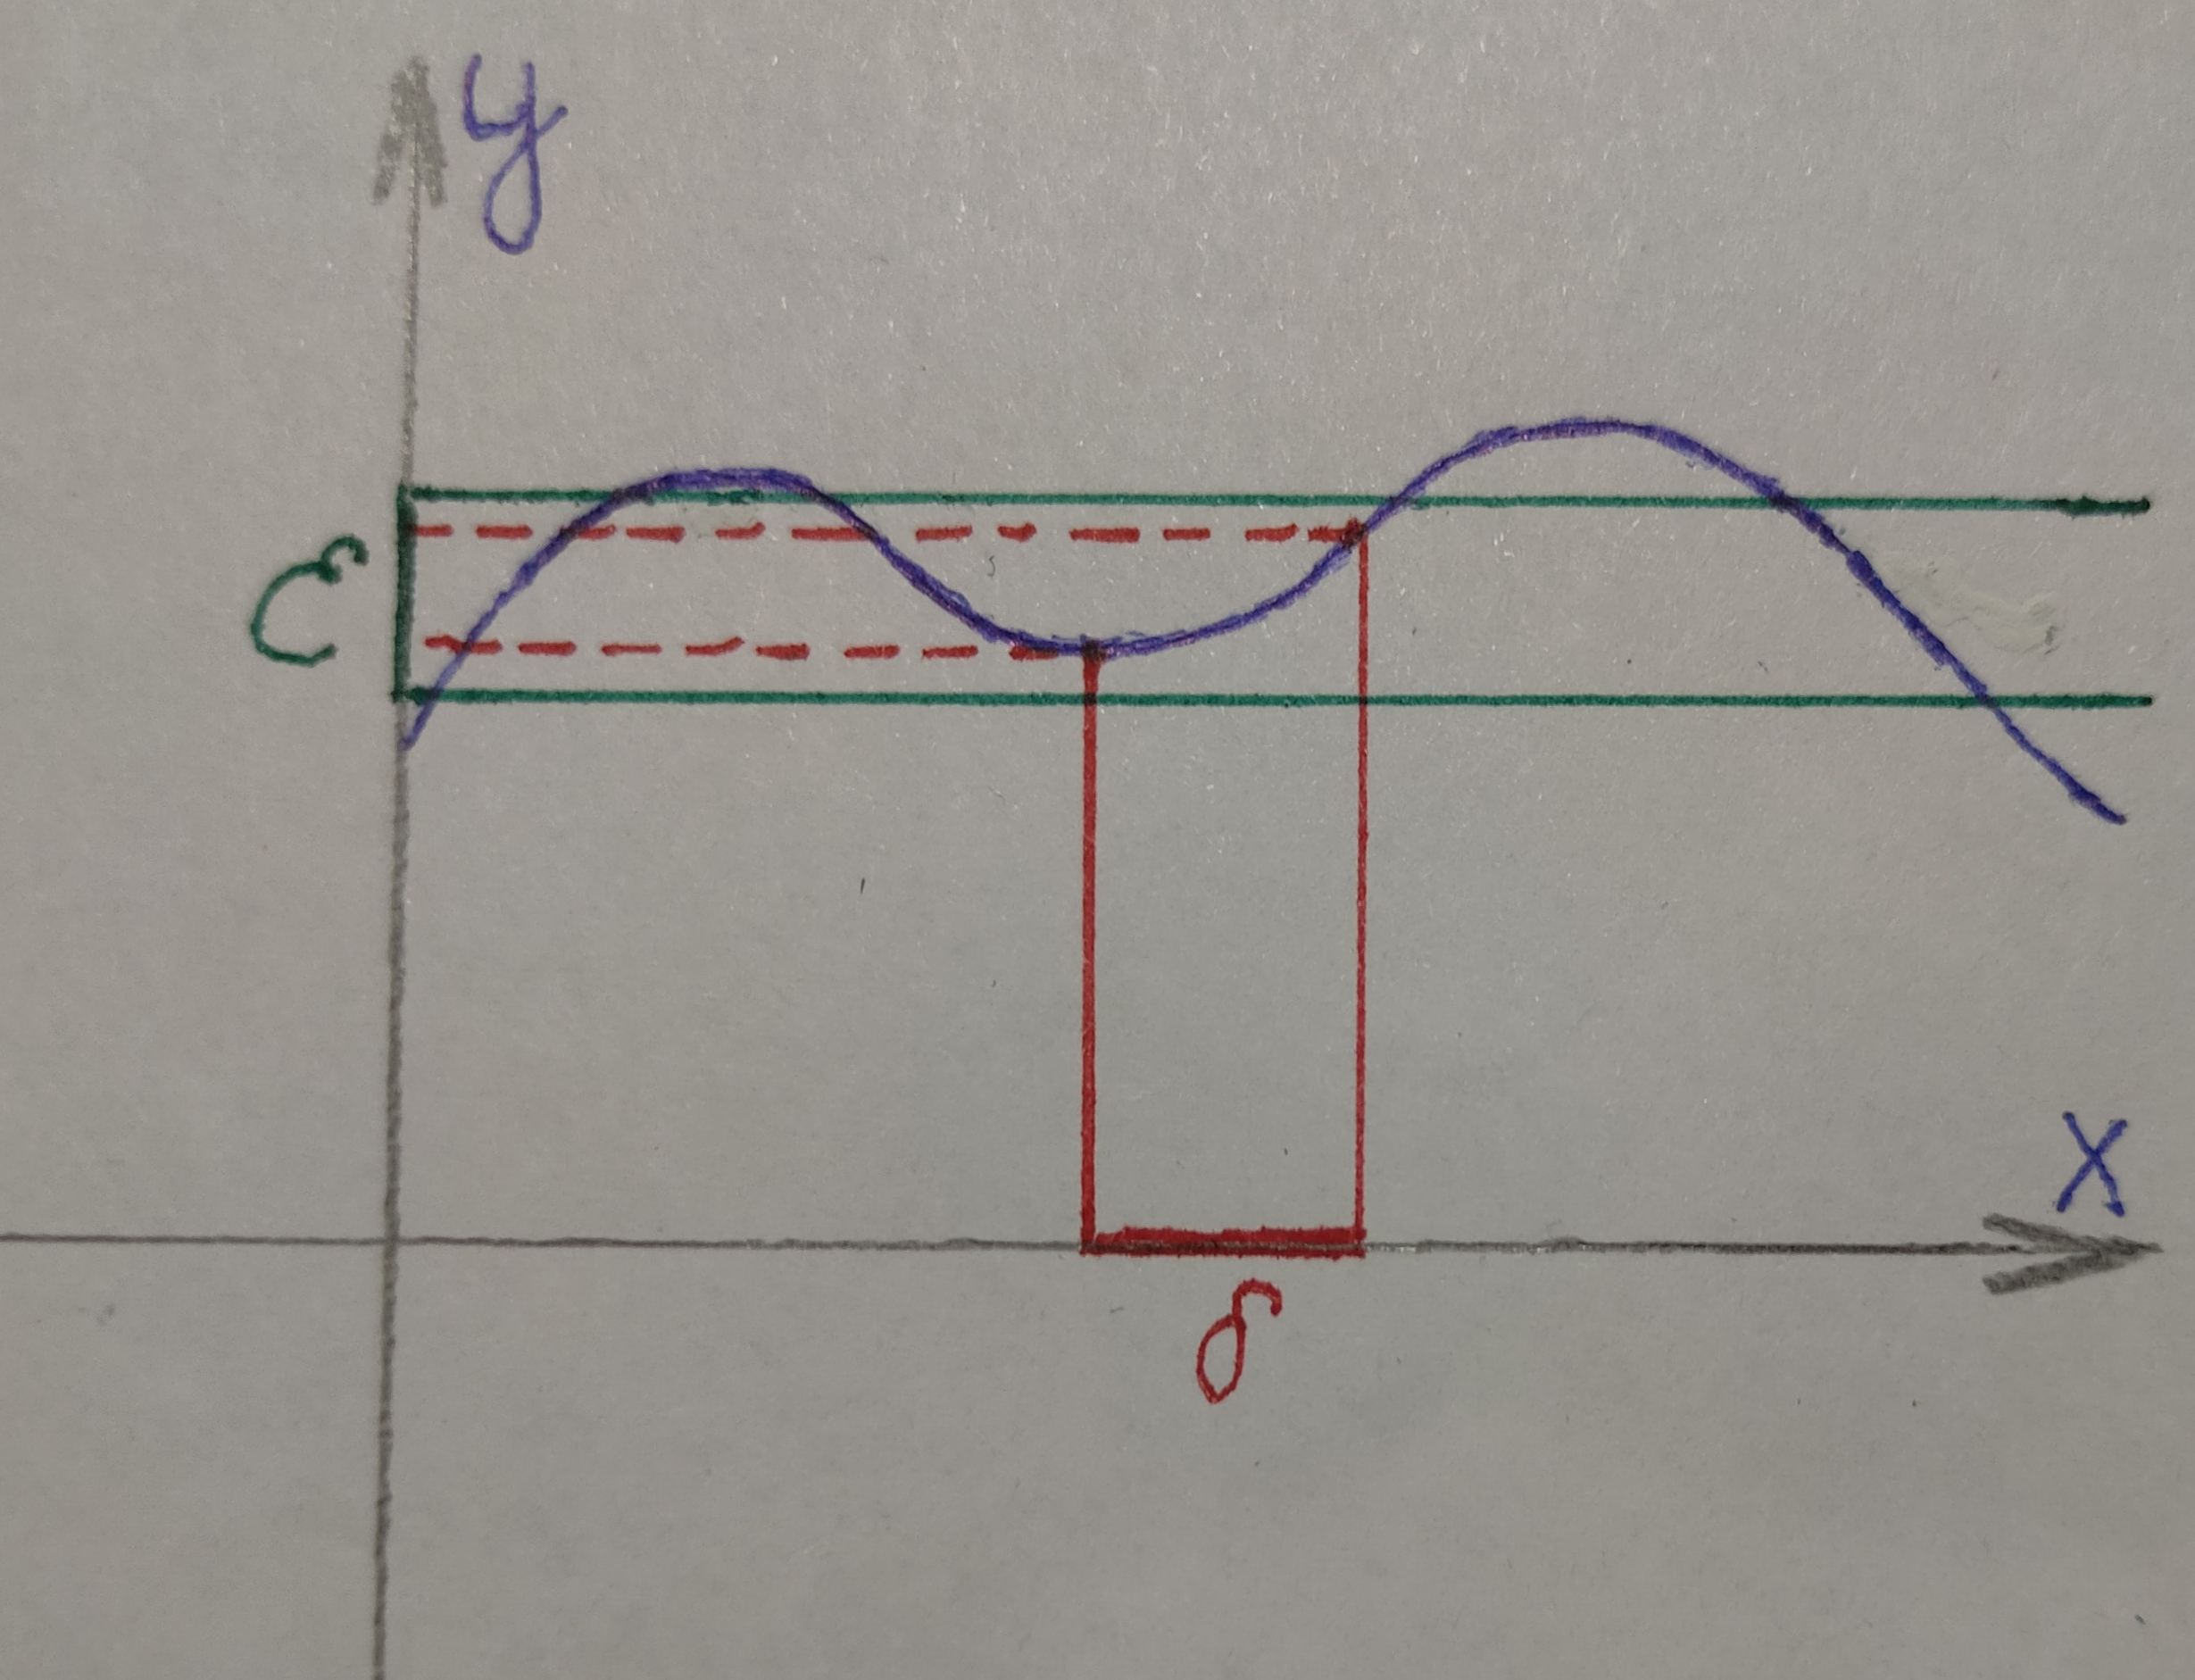
\includegraphics[width=0.5\textwidth]{img/leсture27/uniformly_continuous_function}
    \end{center}
    
    \begin{explanation}
    	Другими словами, существует $\delta$ на оси OX такая, что расстояние между $x$ и $y$ меньше, чем $\delta$, и разность между значениями функции $x$ и $y$ помещается в этот $\epsilon-$корридор.
    \end{explanation}
    
    \begin{mention}
    	Если функция является равномерно-непрерывной, то она является и непрерывной, т. к. определение непрерывности слабее:
    	\[ f - \text{непрерывна на } X \Rightarrow \forall x_0 \in X \text{ } \forall \epsilon > 0 \text{ } \exists \delta > 0: \forall x \in B_{\delta}(x_0) \rightarrow |f(x) - f(x_0)| < \epsilon \]
    	
    	В обратную сторону это не правда, см. пункт 2) примера 27.1.
    \end{mention}
    
    \begin{example}
    	\begin{enumerate}
    		\item Функция $f(x) := \sin{x}$ равномерно непрерывна на $\R$, т.к.
    		по теореме Лагранжа $|\sin{x} - \sin{y}| = |\cos{\xi}| \cdot |x - y| \leqslant |x - y|$.
    		\item Функция $f(x) = \frac{1}{x}$ не равномерно непрерывна на $(0, 1)$,
    		т.к. $f(\frac{1}{2n}) - f(\frac{1}{n}) = n, а |\frac{1}{n} - \frac{1}{2n}| = \frac{1}{2n} \rightarrow 0$.
    	\end{enumerate}
    \end{example}
    
    \begin{explanation}
    	\begin{enumerate}
    		\item По теореме Лагранжа $\forall x, y \in \R |\sin{x} - \sin{y}| = |(\sin{\xi})'(x - y)| = |\cos{\xi}||(x - y)| \leqslant |x - y|$
    		\item Требуется доказать отрицание определения равномерной непрерывности:
    		\[ \exists \epsilon = 1 \text{ } \forall \delta > 0 \text{ } \exists x, y \in (0, 1) \text{ } |x - y| < \delta: |f(x) - f(y)| \geqslant 1 \]
    		Будем доказывать для $\delta = \frac{1}{n}$, потому что всегда можно взять $\frac{1}{n} < \delta$. Тогда пусть $x = x_n = \frac{1}{n}, y = y_n = \frac{1}{2n} \Rightarrow |x - y| = |\frac{1}{n} - \frac{1}{2n}| = \frac{1}{2n} < \frac{1}{n}, |f(x) - f(y)| = |n - 2n| = n \geqslant 1$.
    	\end{enumerate}
    \end{explanation}
    
    \subsection{Интегрируемость непрерывной функции}
    
    \begin{theorem}[Кантора]
    	Если функция $f$ непрерывна на отрезке $[a, b]$, то $f$ равномерно непрерывна на $[a, b]$.
    \end{theorem}
    
    \begin{corollary}
    	Пусть $f$ непрерывна на $[a, b]$. Тогда $f$ интегрируема по Риману на $[a, b]$.
    \end{corollary}
    
    \newpage
    
    \section{Лекция 28: Формула Ньютона-Лейбница}
    
    \subsection{Аддитивность интеграла}
    
    \begin{corollary}
    	Если $f$ интегрируема по Риману на отрезке $[a, b]$, $[c, d] \subseteq [a, b]$, то $f$ интегрируема на отрезке $[c, d]$.
    \end{corollary}
    
    \begin{corollary}
    	Если $f$ интегрируема по Риману на отрезке $[a, b]$, $c \in [a, b]$, то $f$ интегрируема на отрезках $[a, c]$ и $[c, b]$ и верно равенство
    	\[ \int_a^b f(x) \; dx = \int_a^c f(x) \; dx + \int_c^b f(x) \; dx. \]
    \end{corollary}
    
    \subsection{Формула Ньютона–Лейбница}
    
    \begin{theorem}[Формула Ньютона–Лейбница]
    	Пусть $F$ - первообразная интегрируемой по Риману на отрезке
    	$[a, b]$ функции $f$. Тогда
    	\[ \int_{a}^{b} f(x) \; dx = F(b) - F(a) = F(x)\bigg|_{a}^{b}. \]
    \end{theorem}
    
    Далее будем использовать соглашение: при $b > a$ по
    определению 
    \[ \displaystyle\int_{b}^{a} f(x) \; dx = -\displaystyle\int_{a}^{b} f(x) \; dx.\]
    
    \subsection{Существование первообразной}
    
    \begin{theorem}
    	Пусть $f$ интегрируема по Риману на $[a, b]$. Тогда функция
    	\[ F(x) := \int_a^{x} f(x) \; dx \]
    	непрерывна на $[a, b]$. Кроме того, если $f$ непрерывна в точке
    	$x_0 \in [a, b]$, то $F$ дифференцируема в $x_0$ и $F'(x_0) = f(x_0)$.
    \end{theorem}
    
    \begin{proof}
    \end{proof}
    
    \begin{corollary}
    	Пусть $f$ непрерывна на $[a, b]$, тогда у $f$ существует
    	первообразная.
    \end{corollary}
    
    \subsection{Формула интегрирования по частям}
    
    \begin{theorem}[Формула интегрирования по частям]
    	Пусть $f$, $g$ — непрерывно дифференцируемые на отрезке $[a, b]$ функции. Тогда
    	\[ \int_a^b f(x)g'(x) \; dx = f(b)g(b) - f(a)g(a) - \int_a^b f'(x)g(x) \; dx. \]
    \end{theorem}
    
    \begin{example}
    	$\displaystyle\int_0^1 \arctg{x} \; dx.$
    \end{example}
    
    \newpage
    
    \section{Лекция 29: Несобственный интеграл}
    
    \subsection{Формула интегрирования подстановкой}
    
    \begin{theorem}
    	Пусть $f$ — непрерывна на $[a, b], \phi: [\alpha, \beta] \rightarrow [a, b]$ — непрерывно дифференцируемая функция. Тогда
    	\[ \int_{\phi(\alpha)}^{\phi(\beta)} f(x) \; dx = \int_{\alpha}^{\beta} f(\phi(t))\phi'(t) \; dt. \]
    \end{theorem}
    
    \begin{example}
    	$\displaystyle\int_0^{\frac{\pi}{4}} \frac{1}{1 + \cos^2{x}} \; dx.$
    \end{example}
    
    \subsection{Мера Жордана (дополнительный материал)}
    Пусть $\Delta$ — параллелепипед в $\R^n$, являющийся декартовым произведением промежутков вида $[a_i, b_i]$, $(a_i, b_i)$, $[a_i, b_i)$ или $(a_i, b_i]$. Мера Жордана параллелепипеда $\Delta$ определяется как
    произведение
    \[ \mu\Delta = \prod_{i = 1}^{n} (b_i - a_i). \]
    
    Для ограниченного множества $E \subset \R^n$ определяются:
    \begin{itemize}
    	\item внешняя мера Жордана
    	\[ \mu^{*}E = \inf{\sum_{k = 1}^{N} \mu \Delta_k}, \text{   } \bigcup_k{\Delta_k} \supset E \]
    	\item внутренняя мера Жордана
    	\[ \mu_{*}E = \sup{\sum_{k = 1}^{N} \mu \Delta_k}, \bigcup_k{\Delta_k} \subset E, \Delta_k \cap \Delta_m = \varnothing, \text{ если } k \neq m. \]
    \end{itemize}
    
    Здесь $\Delta_1, \Delta_2, ..., \Delta_N$ — параллелепипеды описанного выше вида.
    
    \begin{definition}
    	Множество $E$ называется измеримым по Жордану (или
    	квадрируемым), если $\mu^{*}E = \mu_{*}E$. В этом случае мера Жордана равна $\mu E = \mu^{*}E = \mu_{*}E$.
    \end{definition}
    
    \subsection{Несобственный интеграл Римана}
    
    \begin{definition}
    	Пусть $f$ интегрируема на каждом отрезке $[a, x]$ при $x < b$ $(b \in (-\infty, +\infty])$. Говорят, что несобственный интеграл
    	\[ \int_a^b f(t) \; dt \]
    	\underline{сходится}, если существует предел
    	\[ \lim_{x \to b - 0} \int_a^x f(t) \; dt. \]
    
	    В этом случае значение несобственного интеграла полагают
	    равным значению данного предела. В противном случае (если
	    предела не существует) говорят, что несобственный интеграл
	    \underline{расходится}.
	    
	    Аналогично определяется несобственный интеграл с
	    особенностью в нижнем пределе интегрирования.
	\end{definition}
	
	\begin{example}
	    \begin{equation*}
	    	\int_1^b \frac{1}{x^p} \; dt = 
		    \begin{cases}
		    	\frac{1}{1 - p}(b^{1 - p} - 1), & p \neq 1, \\
		    	\ln{b}, & p = 1.
		    \end{cases}
	    \end{equation*}
	    
	    Предел при $b \rightarrow \infty$ существует тогда и только тогда, когда $p > 1$.
	    
	    С другой стороны,
	    \begin{equation*}
	    	\int_b^1 \frac{1}{x^p} \; dt = 
	    	\begin{cases}
	    		\frac{1}{1 - p}(1 - b^{1 - p}), & p \neq 1, \\
	    		-\ln{b}, & p = 1.
	    	\end{cases}
	    \end{equation*}
	    
	    Предел при $b \rightarrow 0$ существует тогда и только тогда, когда $p < 1$.
	\end{example}
	
	\subsection{Свойства несобственного интеграла}
	
	\begin{theorem}
		Пусть $f$, $g$ интегрируемы на каждом отрезке $[a, x]$ при $x < b$ и пусть для них определены несобственные интегралы на
		промежутке $[a, b)$. Тогда
		\begin{enumerate}
			\item если $b \in \R$ и $f$ интегрируема на $[a, b]$, то значение несобственного интеграла на промежутке $[a, b)$ совпадает со значением обычного интеграла Римана по отрезку $[a, b]$;
			\item функция $\alpha f + \beta g$ интегрируема в несобственном смысле на промежутке $[a, b)$ и
			\[ \int_a^b (\alpha f + \beta g) \; dx = \alpha \int_a^b f(x) \; dx + \beta \int_a^b g(x) \; dx; \]
			\item если $c \in [a, b)$, то
			\[ \int_a^b f(x) \; dx = \int_a^c f(x) \; dx + \int_c^b f(x) \; dx; \]
		\end{enumerate}
	\end{theorem}
	
	\subsection{Формула интегрирования подстановкой}
	
	\begin{theorem}
		Пусть $f$ непрерывна на $[a, b)$, $\phi: [\alpha, \beta) \rightarrow [a, b)$ - непрерывно дифференцируемое отображение, $\phi(\alpha) = a, \phi(t) \rightarrow b$ при
		$t \rightarrow \beta$. Тогда функция $t \mapsto f(\phi(t))\phi'(t)$ интегрируема в несобственном смысле на промежутке $[\alpha, \beta)$ и
		\[ \int_a^b f(x) \; dx = \int_{\alpha}^{\beta} f(\phi(t))\phi'(t) \; dt. \]
	\end{theorem}
	
	\subsection{Формула интегрирования по частям}
	
	\begin{theorem}
		Пусть $f, g$ непрерывно дифференцируемы на $[a, b)$ и существует предел $\displaystyle\lim_{x \to b - 0} f(x)g(x)$. Тогда функции $f'g$ и $fg'$ одновременно интегрируемы или не интегрируемы в несобственном смысле на $[a, b)$ и в случае интегрируемости
		\[ \int_a^b f(t)g'(t) \; dt = \lim_{x \to b - 0} f(x)g(x) - f(a)g(a) - \int_a^b f(t)g'(t) \; dt. \]
	\end{theorem}
	
	\subsection{Критерий Коши}
	
	\begin{theorem}[Критерий Коши]
		Пусть функция $f(x)$ определена на промежутке $[a; b)$,
		интегрируема в собственном смысле на любом отрезке
		$[a; \xi] \subseteq [a; b)$ и неограниченна в левой окрестности точки $x = b$. Тогда для сходимости интеграла
		\[ \int_a^b f(x) \; dx \]
		необходимо и достаточно, чтобы для любого числа $\epsilon > 0$
		существовало такое число $\eta$, что при любых $\eta_1, \eta_2 \in (\eta; b)$
		\[ \bigg| \int_{\eta_1}^{\eta_2} f(x) \; dx \bigg| < \epsilon. \]
	\end{theorem}
	
	\newpage
	
	\section{Лекция 30: Абсолютная сходимость}
	
	\subsection{Абсолютная сходимость}
	
	\begin{definition}
		Говорят, что несобственный интеграл $\displaystyle \int_a^b f(t) \; dt$ сходится \textbf{абсолютно}, если сходится интеграл $\displaystyle \int_a^b |f(t)| \; dt$.
	\end{definition}
	
	\begin{sentence}
		Из абсолютной сходимости интеграла следует обычная сходимость.
	\end{sentence}
	
	\begin{proof}
	\end{proof}
	
	\begin{mention}
		Исследование абсолютной сходимости сводится к исследованию сходимости интеграла от неотрицательной функции. В случае неотрицательной функции $f$ функция $F$ оказывается монотонной, поэтому сходимость интеграла от неотрицательной функции равносильна ограниченности $F$ на $[a, b)$.	
	\end{mention}
	
	\subsection{Условная сходимость}
	
	\begin{definition}
		Говорят, что несобственный интеграл $\int_a^b f(t) \; dt$ сходится \textbf{условно}, если сам интеграл сходится, но не сходится
		абсолютно.
	\end{definition}
	
	\begin{example}
		\[ \int_1^{\infty} \frac{\sin{x}}{x} \; dx = -\frac{\cos{x}}{x} \bigg|_1^{\infty} - \int_1^{\infty} \frac{\cos{x}}{x^2} \; dx, \]
		последний интеграл сходится абсолютно. В то же время,
		\[ \int_1^{\infty} \bigg|\frac{\sin{x}}{x}\bigg| \; dx \geqslant \int_1^{\infty} \frac{\sin^2{x}}{x} \; dx = \int_1^{\infty} \frac{1}{2x} - \frac{\cos{2x}}{2x} \; dx, \]
		где первый интеграл не сходится, а второй сходится, а значит и интеграл от суммы сходиться не может.
	\end{example}
	
	\subsection{Несобственный интеграл от знакопостоянной функции}
	
	\begin{theorem}[Критерий сходимости несобственного
		интеграла от знакопостоянной функции]
		Пусть функция $f(x) \geqslant 0$ интегрируема на любом отрезке
		$[a, b'] \subset [a, b)$. Тогда сходимость интеграла $\displaystyle \int_a^b f(x) \; dx$	эквивалентна условию $\displaystyle \sup_{b' \in [a, b)} {\int_a^{b'} f(x) \; dx < +\infty}$.
	\end{theorem}
	
	\begin{proof}
	\end{proof}
	
	\subsection{Первый признак сравнения}
	
	\begin{theorem}[Первый признак сравнения]
		Пусть функции $f(x)$ и $g(x)$ интегрируемы на любом отрезке
		$[a, b'] \subset [a, b)$ и для любого $x \in [a, b)$ $0 \leqslant f(x) \leqslant g(x)$. Тогда:
		\begin{itemize}
			\item из сходимости $\displaystyle$ следует сходимость;
			\item из расходимости следует расходимость.
		\end{itemize}
	\end{theorem}
	
	\begin{proof}
	\end{proof}
	
	\subsection{Эквивалентность в смысле сходимости интегралов}
	
	\begin{definition}
		Будем говорить, что $f(x)$ и $g(x)$ эквивалентны в смысле
		сходимости интегралов при $x \rightarrow b - 0$ (обозн. $f(x) \overset{\text{сх.}}{\sim} g(x)$ при $x \rightarrow b - 0$), если $\exists m, M > 0, b_1 < b$ такие, что $\forall x \in [b_1, b)$ выполняются неравенства
		\[ mg(x) \leqslant f(x) \leqslant Mg(x).\]
	\end{definition}
	
	\begin{theorem}[Второй признак сравнения]
		Пусть неотрицательные функции $f(x)$ и $g(x)$ интегрируемы на
		любом отрезке $[a, b'] \subset [a, b)$ и $f(x) \overset{\text{сх.}}{\sim} g(x)$ при $x \rightarrow b - 0$.
		
		Тогда несобственные интегралы $\int_a^b g(x) \; dx$ и $\int_a^b а(x) \; dx$ сходятся и расходятся одновременно.
	\end{theorem}
	
	\begin{proof}
	\end{proof}
	
	\subsection{Второй признак сравнения}
	
	\begin{sentence}
		Если $f \geqslant 0$ и $f(x) \sim g(x)$ при $x \rightarrow b - 0$, то $f(x) \overset{\text{сх.}}{\sim} g(x)$.
	\end{sentence}
	
	\begin{proof}
	\end{proof}
	
	\begin{sentence}
		Пусть $f_i(x), g_i(x)$ $i \in \{1, 2, 3\}$ - неотрицательные на
		промежутке $[a, b)$ функции, причем $f_3(x) > 0, g_3(x) > 0$ и
		$f_i(x) \overset{\text{сх.}}{\sim} g_i(x)$ $i \in \{1, 2, 3\}$ при $x \rightarrow b - 0$. Тогда
		\[ \frac{f_1(x) \cdot f_2(x)}{f_3(x)} \overset{\text{сх.}}{\sim} \frac{f_1(x) \cdot f_2(x)}{f_3(x)} \text{ при } x \rightarrow b - 0.\]
	\end{sentence}
	
	\begin{proof}
	\end{proof}
	
	\begin{example}
		Исследовать на сходимость $\displaystyle \int_1^{+\infty} \frac{\arctan{\frac{1}{x}}\sin{(\frac{2 + \cos{x}}{x^2})}}{(e^{\frac{1}{x}} - 1)^{\alpha}} \; dx$.
	\end{example}
	
	\newpage
	
	\section{Лекция 31: Еще немного про числовые ряды}
	
	\subsection{Первый признак сравнения}
	
	\begin{definition}
		Ряд $\sum_{n = 1}^{\infty} a_n$ называется \textbf{знакопостоянным}, если или
		$a_n \geqslant 0 \text{ } \forall n \in \N$, или $a_n \leqslant 0 \text{ } \forall n \in \N$.
	\end{definition}
	
	\begin{sentence}[Первый признак сравнения]
		Пусть $0 \leqslant a_n \leqslant b_n$. Если ряд $\displaystyle \sum_{k = 1}^{\infty} b_k$ сходится, то сходится и ряд $\displaystyle \sum_{k = 1}^{\infty} a_k$. Наоборот, если ряд $\displaystyle \sum_{k = 1}^{\infty} a_k$ расходится, то расходится и ряд $\displaystyle \sum_{k = 1}^{\infty} b_k$.
	\end{sentence}
	
	\begin{proof}
	\end{proof}
	
	\begin{mention}
		Поскольку первые несколько членов не влияют на сходимость
		ряда, достаточно, чтобы неравенства выше выполнялись
		начиная с некоторого момента $\forall n > n_0$. Это называется
		\textbf{принципом локализации}.
	\end{mention}
	
	\begin{corollary}[Признак Вейерштрасса]
		Если $|a_n| \leqslant b_n$ и ряд $\displaystyle \sum_{n = 1}^{\infty} b_n$ сходится, то ряд $\displaystyle \sum_{n = 1}^{\infty} a_n$ сходится.
	\end{corollary}
	
	\subsection{Второй признак сравнения}
	
	\begin{theorem}[Второй признак сравнения]
		Пусть $a_n, b_n > 0$ и $\displaystyle \exists \lim_{n \to \infty} {\frac{a_n}{b_n}} = c \neq 0$. Тогда $\displaystyle \sum_{n = 1}^{\infty} a_n \sim \sum_{n = 1}^{\infty} b_n -$ эквивалентны по сходимости, т.е. сходятся/расходятся одновременно.
	\end{theorem}
	
	\begin{proof}
	\end{proof}
	
	\begin{corollary}
		Если $a_n \geqslant 0$ и $a_n \sim b_n, n \rightarrow \infty, $ то $\displaystyle \sum_{n = 1}^{\infty} a_n \sim \sum_{n = 1}^{\infty} b_n$.
	\end{corollary}
	
	\subsection{Интегральный признак}
	
	\begin{sentence}
		Пусть $f(x) \leqslant 0$ и не возрастает на промежутке $[1, +\infty)$. Тогда ряд $\displaystyle \sum_{n = 1}^{\infty} f(n)$ и интеграл $\displaystyle \int_1^{+\infty} f(x) \; dx$ сходятся и расходятся одновременно. 
	\end{sentence}
	
	\begin{proof}
	\end{proof}
	
	\begin{example}
		Ряд $\displaystyle \sum_{n = 1}^{\infty} \frac{1}{n^p}$ сходится при $p > 1$ и расходится при $p \leqslant 1$.
	\end{example}
	
	\subsection{Признак Даламбера}
	
	\begin{theorem}[Признак Даламбера]
		Пусть $a_k > 0$ $\forall k \in \N$. Тогда
		\begin{enumerate}
			\item если существует $k_0 \in \N$ и $q \in (0, 1)$ такие, что $\frac{a_{k + 1}}{a_k} \leqslant q$ $\forall k \geqslant k_0,$ то ряд $\displaystyle \sum_{k = 1}^{\infty} a_k$ сходится;
			\item если $\exists k_0 : \forall k \leqslant k_0 \rightarrow \frac{a_{k + 1}}{a_k} \geqslant 1$, то ряд $\displaystyle \sum_{k = 1}^{\infty} a_k$ расходится.
		\end{enumerate}
	\end{theorem}
	
	\begin{proof}
	\end{proof}
	
	\begin{corollary}[Признак Даламбера в предельной форме]
		Пусть $a_k > 0$ $\forall k \in \N$ и $\displaystyle \lim_{k \to \infty} {\frac{a_{k + 1}}{a_k}} = q$, тогда
		
		\begin{enumerate}
			\item при $q < 1$ ряд $\displaystyle \sum_{k = 1}^{\infty} {a_k}$ сходится;
			\item при $q > 1$ ряд $\displaystyle \sum_{k = 1}^{\infty} {a_k}$ расходится;
			\item при $q = 1$ ряд $\displaystyle \sum_{k = 1}^{\infty} {a_k}$ может сходится, а может и расходится.
		\end{enumerate}
	\end{corollary}
	
	\subsection{Радикальный признак Коши}
	
	\begin{theorem}[Радикальный признак Коши]
		Пусть $a_k > 0$ $\forall k \in \N$. Тогда
		\begin{enumerate}
			\item если существуют $k_0 \in \N$ и $q \in (0, 1)$ такие, что $\sqrt[k]{a_k} \leqslant q$ $\forall k \geqslant k_0$, то ряд $\displaystyle \sum_{k = 1}^{\infty} {a_k}$ сходится;
			\item если $\exists k_0: \forall k \geqslant k_0 \rightarrow \sqrt[k]{a_k} \geqslant 1$, то ряд $\displaystyle \sum_{k = 1}^{\infty} {a_k}$ расходится.
		\end{enumerate}
	\end{theorem}
	
	\begin{proof}
	\end{proof}
	
	\begin{corollary}[Признак Коши в предельной форме]
		Пусть $a_k > 0$ $\forall k \in \N$ и $\displaystyle \lim_{k \to \infty} {\sqrt[k]{a_k}} = q$, тогда
		
		\begin{enumerate}
			\item при $q < 1$ ряд $\displaystyle \sum_{k = 1}^{\infty} {a_k}$ сходится;
			\item при $q > 1$ ряд $\displaystyle \sum_{k = 1}^{\infty} {a_k}$ расходится;
			\item при $q = 1$ ряд $\displaystyle \sum_{k = 1}^{\infty} {a_k}$ может сходится, а может и расходится.
		\end{enumerate}
	\end{corollary}
	
	\begin{example}
		Признак Коши сложнее, однако сильнее, чем признак Даламбера. Если признак Даламбера подтверждает сходимость или расходимость ряда, то и признак Коши делает то же, однако обратное неверно:
		\[ ??????? \sum_{k = 1}^{\infty} {(-1)^p} \]
	\end{example}
	
	\subsection{Признак Гаусса}
	
	\begin{theorem}[Признак Гаусса]
		Пусть $a_n > 0$. Если существует $p \in \R, \delta > 0$ такие, что $\frac{a_{n + 1}}{a_n} = 1 - \frac{p}{n} + O(\frac{1}{n^{1 + \delta}})$, то $\displaystyle \sum_{n = 1}^{\infty} a_n \sim \sum_{n = 1}^{\infty} {\frac{1}{n^p}}$, т. е. при $p > 1$ сходится и при $p \leqslant 1$ расходится.
	\end{theorem}
	
	\begin{proof}
	\end{proof}
	
	\section{Лекция 32: Признаки Абеля и Дирихле}
	
	\subsection{Признак Дирихле}
	
	\begin{theorem}[Признак Дирихле]
		Пусть последовательность частичных сумм ряда $\displaystyle \sum_{k = 1}^{\infty} {a_k}$ ограничена:
		\[ \exists C \in \R: \forall n \in \N \rightarrow \bigg|\sum_{k = 1}^n {a_k}\bigg| \leqslant C, \]
		а последовательность $\{b_k\}$ монотонно стремится к нулю. Тогда ряд $\displaystyle \sum_{k = 1}^{\infty} a_k b_k$ сходится.
	\end{theorem}
	
	\begin{proof}
	\end{proof}
	
	\subsection{Признак Абеля}
	
	\begin{theorem}[Признак Абеля]
		Пусть ряд $\displaystyle \sum_{k = 1}^{\infty} {a_k}$ сходится, последовательность $\{b_k\}$ монотонна и ограничена. Тогда ряд $\displaystyle \sum_{k = 1}^{\infty} a_k b_k$ сходится.
	\end{theorem}
	
	\begin{proof}
	\end{proof}
	
	\begin{corollary}[Следствие из признака Абеля]
		Пусть последовательность $\{b_k\}$ монотонна и $\displaystyle \lim_{k \to \infty} {b_k} = b \in (0, +\infty)$. Тогда ряды $\displaystyle \sum_{k = 1}^{\infty} a_k$ и $\displaystyle \sum_{k = 1}^{\infty} a_k b_k$ сходится или расходятся одновременно.
	\end{corollary}
	
	\begin{mention}
		Следствие из признака Абеля утверждает, что характер
		сходимости ряда $\sum_{k = 1}^{\infty} {a_k}$ не изменится, если последовательность $\{a_k\}$ заменить на эквивалентную последовательность $\{c_k\}$ при условии, что последовательность $\{\frac{c_k}{a_k}\}$ монотонна.
	\end{mention}
	
	\subsection{Признак Лейбница}
	
	\begin{theorem}[Признак Лейбница]
		Если последовательность ${b_k}$ монотонно стремится к нулю, то
		ряд Лейбница $\displaystyle \sum_{k = 1}^{\infty} (-1)^k b_k$ сходится.
	\end{theorem}
	
	\begin{proof}
	\end{proof}
	
	\begin{mention}
		Из того, что ряд $\displaystyle \sum_{k = 1}^{\infty} {a_k}$ сходится и $\displaystyle \lim_{k \to \infty} {\frac{b_k}{a_k}} = 1$ не следует, что $\displaystyle \sum_{k = 1}^{\infty} {b_k}$ сходится.
	\end{mention}
	
    \subsection{Теоремы о среднем}
    
    \begin{theorem}[Первая теорема о среднем]
    	Пусть функции $f(x)$ и $g(x)$ интегрируемы на отрезке $[a; b]$,
    	$m \leqslant f(x) \leqslant M$, и $g(x)$ не меняет знак (то есть либо всюду неотрицательна: $g(x) \geqslant 0$, либо всюду неположительна $g(x) \leqslant 0$). Тогда существует такое число $\mu, m \leqslant \mu \leqslant M$, что
    	\[ \int_a^b f(x)g(x) \; dx = \mu \int_a^b g(x) \; dx. \]
    \end{theorem}
    
    \begin{proof}
    \end{proof}
    
    \begin{corollary}[Первая теорема о среднем]
    	Пусть функции $f(x)$ - непрерывна, а $g(x)$ интегрируема на отрезке $[a; b]$ и не меняет знак. Тогда существует такое число
    	$c \in [a, b]$, что
    	\[ \int_a^b f(x)g(x) \; dx = f(с) \int_a^b g(x) \; dx. \]
    \end{corollary}
    
    \begin{theorem}[Вторая теорема о среднем]
    	Если функция $f(x)$ монотонна (нестрого) на отрезке $[a, b]$, а
    	функция $g(x)$ интегрируема на $[a, b]$, то существует точка
    	$\xi \in [a, b]$ такая, что
    	\[ \int_a^b f(x)g(x) \; dx = f(a) \int_a^{\xi} g(x) \; dx + f(b) \int_{\xi}^b g(x) \; dx. \]
    \end{theorem}
    
    \begin{proof}
    \end{proof}
    
    \begin{lemma}[Формулы Бонне]
    	Если функция $f(x)$ не возрастает и $f(x) \geqslant 0$ на отрезке $[a, b]$, а функция $g(x)$ интегрируема на $[a, b]$, то существует точка $\xi \in [a, b]$ такая, что
    	\[ \int_a^b f(x)g(x) \; dx = f(a) \int_a^{\xi} g(x) \; dx. \]
    	Если же функция $f(x)$ не убывает, то
    	\[ \int_a^b f(x)g(x) \; dx = f(b) \int_{\xi}^b g(x) \; dx. \]
    \end{lemma}
    
    \subsection{Признак Дирихле}
    
    Пусть функция $y = f(x)g(x)$ определена на промежутке $[a; b)$ и
    неограниченна в левой окрестности точки $x = b$. Тогда справедливы следующие достаточные признаки сходимости.
    
    \begin{theorem}[Признак Дирихле]
    	Интеграл $\int_a^b f(x)g(x) \; dx$ сходится, если:
    	\begin{itemize}
    		\item функция $f(x)$ непрерывна и имеет ограниченную
    		первообразную на $[a; b)$;
    		\item функция $g(x)$ монотонна на $[a; b)$, причем $\displaystyle \lim_{x \to b - 0} {g(x)} = 0$.
    	\end{itemize}
    \end{theorem}
    
    \begin{example}
    	Интеграл $\displaystyle \int_1^{+\infty} {\frac{\sin{x}}{x^a}} \; dx$, сходится при $\alpha > 0$ по признаку Дирихле.
    \end{example}
    
    \subsection{Признак Абеля}
    
    В условиях предыдущего слайда на функцию $y = f(x)g(x)$ справедлив следующий достаточный признак сходимости.
    
    \begin{theorem}[Признак Абеля]
    		Интеграл $\int_a^b f(x)g(x) \; dx$ сходится, если:
    	\begin{itemize}
    		\item функция $f(x)$ непрерывна на $[a; b)$ и интеграл $\int_a^b f(x) \; dx$ сходится;
    		\item функция $g(x)$ ограничена и монотонна на $[a; b)$.
    	\end{itemize}
    \end{theorem}
    
    \begin{example}
    	Докажите, что при $\alpha > 0$ интеграл $\displaystyle \int_1^{+\infty} \frac{\sin{x}}{x^{\alpha}} \arctan{x} \; dx$ сходится.
    \end{example}
	
\end{document}
